
% =========================
% 1. Overview
% =========================

\begin{frame}{Learning Outcomes}
    \begin{itemize}
        \item Explain the core components of the ML framework and how they differ from traditional programming.

        \item Identify data problems and model failures using loss curves.
        
        \item Select appropriate data splitting strategies (Stratified K-Fold) to simulate unseen data.
        
        \item Select and justify the appropriate metrics based on data characteristics.
        
        \item Understand essential preprocessing techniques including cleaning, scaling, and feature selection to optimize model performance.
    \end{itemize}
\end{frame}

% --- TABLE OF CONTENTS ---
\begin{frame}{Table of Contents}
    \tableofcontents
\end{frame}

% =========================
% 2. The Mental Model (Components)
% =========================

\section{What is Machine Learning?}

\subsection{Introduction}

\begin{frame}{What is Machine Learning?}
    % Top definition
    \textbf{Machine Learning} is the field of study that gives computers the ability to learn (using data) without being explicitly programmed.
    \vspace{1.5em}

    \begin{columns} % T aligns columns at the top
        % Left Column: Traditional
        \begin{column}{0.48\textwidth}
            \centering            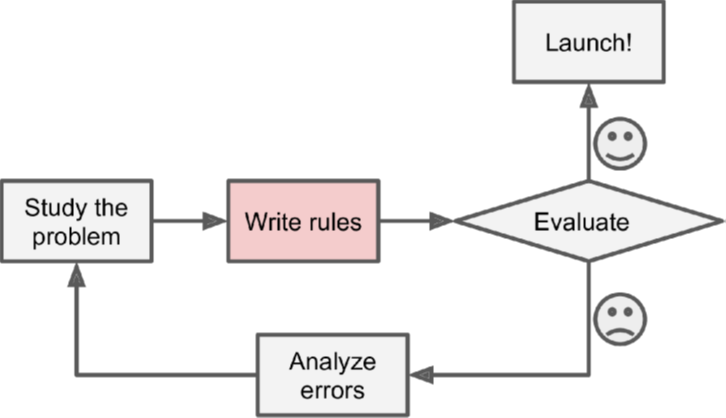
\includegraphics[width=1.0\linewidth]{images/traditional.png} 
            \vspace{1em}
            \textit{The traditional approach} \\
            % \vspace{0.5em}
            \textbf{Rules + Data = Answers}
        \end{column}
        % Right Column: Machine Learning
        \begin{column}{0.48\textwidth}
            \centering
            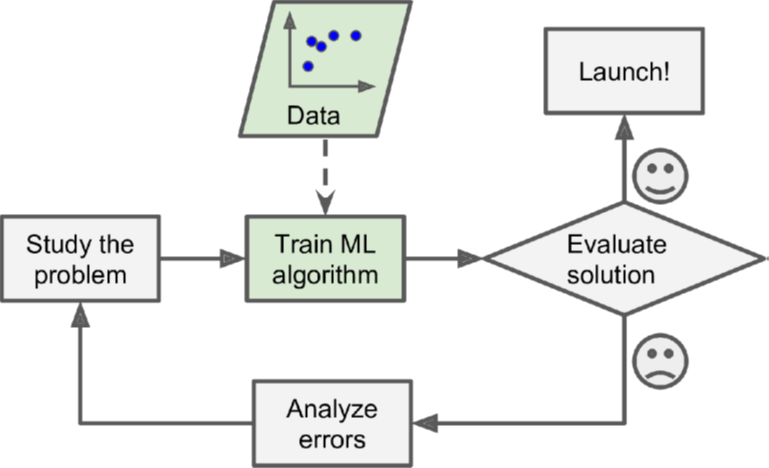
\includegraphics[width=1.0\linewidth]{images/ml.png} 
            \vspace{1em}
            \textit{The Machine Learning approach} \\
            % \vspace{0.5em}
            \textbf{Data + Answers = Rules}
        \end{column}
    \end{columns}
\end{frame}


\begin{frame}{Data Types}
    \begin{columns}[T]
        % --- Column 1: Structured Data ---
        \begin{column}{0.48\textwidth}
            \textbf{\large 1. Structured Data} \\
            \vspace{0.3em}
            \textit{Organized in rows and columns.}
            \vspace{0.8em}
            
            \begin{itemize}
                \setlength\itemsep{0.8em}
                \item \textbf{Tabular Data}
                \begin{itemize}
                    \item Spreadsheets, SQL Databases
                    \item \textit{Columns = Features, Rows = Samples}
                \end{itemize}
                \item \textbf{Time-Series Data}
                \begin{itemize}
                    \item Data indexed by time
                    \item Stock prices, Weather, IoT sensors
                \end{itemize}
            \end{itemize}
        \end{column}

        % --- Column 2: Unstructured Data ---
        \begin{column}{0.48\textwidth}
            \textbf{\large 2. Unstructured Data} \\
            \vspace{0.3em}
            \textit{Complex formats.}
            \vspace{0.8em}

            \begin{itemize}
                \setlength\itemsep{0.8em}
                \item \textbf{Text Data (NLP)}
                \begin{itemize}
                    \item Emails, Tweets, Documents
                \end{itemize}
                \item \textbf{Images \& Video (Computer Vision)}
                \begin{itemize}
                    \item Medical imaging, Surveillance, Face ID
                \end{itemize}
                \item \textbf{Audio Data}
                \begin{itemize}
                    \item Voice commands, Music processing
                \end{itemize}
            \end{itemize}
        \end{column}
    \end{columns}
    \textbf{Note:} \textit{Machine Learning excels at Structured Data, while Deep Learning dominates Unstructured Data.}
\end{frame}

\begin{frame}{Types of Machine Learning}
    \begin{block}{1. Supervised Learning}
        We have input data $X$ and corresponding target labels $y$.
        The goal is to learn a mapping $f(x) \approx y$.
    \end{block}
    \vspace{1em}

    \begin{columns}[T]
        % --- Regression ---
        \begin{column}{0.48\textwidth}
        \centering
            \textbf{\medium A. Regression} \\
            \textit{Predicting continuous values (e.g., Price)}
            \vspace{1em}
            \centering
            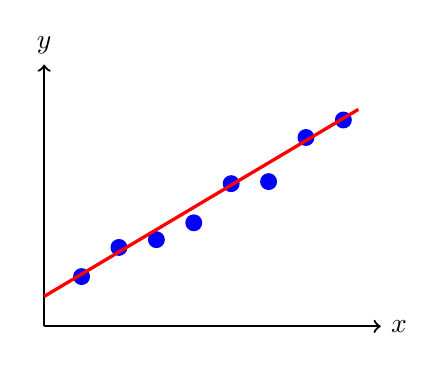
\begin{tikzpicture}[scale=0.95]
                % Axes
                \draw[->, thick] (0,0) -- (4.5,0) node[right] {$x$};
                \draw[->, thick] (0,0) -- (0,3.5) node[above] {$y$};
                % Data Points
                \foreach \x in {0.5,1,1.5,2,2.5,3,3.5,4} 
                    \filldraw [blue] (\x, 0.6*\x + 0.4 + 0.3*rand) circle (3pt);
                % Regression Line
                \draw [red, very thick] (0,0.4) -- (4.2,2.9);
            \end{tikzpicture}
        \end{column}

        % --- Classification ---
        \begin{column}{0.48\textwidth}
        \centering
            \textbf{\medium B. Classification} \\
            \textit{Predicting discrete categories (e.g., Spam Classification)}
            \vspace{1em}
            \centering
            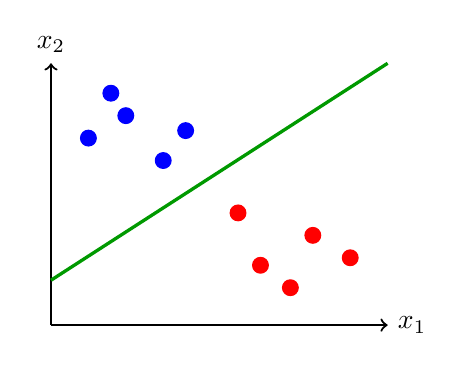
\begin{tikzpicture}[scale=0.95]
                % Axes
                \draw[->, thick] (0,0) -- (4.5,0) node[right] {$x_1$};
                \draw[->, thick] (0,0) -- (0,3.5) node[above] {$x_2$};
                % Class 0 (Blue Circles)
                \foreach \p in {(0.5,2.5), (1,2.8), (1.5,2.2), (0.8,3.1), (1.8,2.6)} 
                    \filldraw [blue] \p circle (3pt);
                % Class 1 (Red Squares - visually circles here for simplicity)
                \foreach \p in {(2.8,0.8), (3.5,1.2), (3.2,0.5), (4,0.9), (2.5,1.5)} 
                    \filldraw [red] \p circle (3pt);
                % Decision Boundary
                \draw [green!60!black, very thick] (0,0.6) -- (4.5,3.5);
            \end{tikzpicture}
        \end{column}
    \end{columns}
\end{frame}

\begin{frame}{Types of Machine Learning}
    \begin{block}{2. Unsupervised Learning}
        We only have input data $X$ (No labels). 
        The goal is to discover hidden structures or patterns.
    \end{block}
    \vspace{1em}

    \begin{columns}[T]
        % --- Clustering ---
        \begin{column}{0.48\textwidth}
        \centering
            \textbf{\medium A. Clustering (Grouping)} \\
            \textit{Grouping similar examples (e.g., customers segmentation)}
            \vspace{1em}
            \centering
            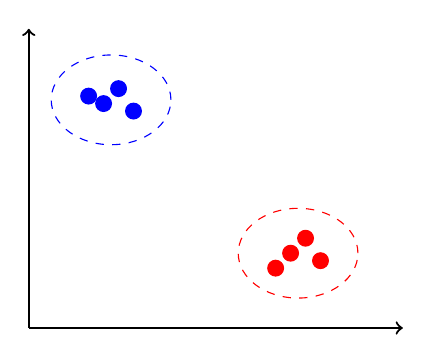
\begin{tikzpicture}[scale=0.95]
                % Fixed Axis Size for consistency
                \draw[->, thick] (0,0) -- (5,0);
                \draw[->, thick] (0,0) -- (0,4);
                
                % Cluster 1 (Top Left)
                \foreach \p in {(1,3), (1.2,3.2), (0.8,3.1), (1.4,2.9)} 
                    \filldraw [blue] \p circle (3pt);
                \draw [blue, dashed] (1.1,3.05) ellipse (0.8cm and 0.6cm);
                
                % Cluster 2 (Bottom Right)
                \foreach \p in {(3.5,1), (3.7,1.2), (3.3,0.8), (3.9,0.9)} 
                    \filldraw [red] \p circle (3pt);
                \draw [red, dashed] (3.6,1) ellipse (0.8cm and 0.6cm);
            \end{tikzpicture}
        \end{column}

        % --- Dimensionality Reduction ---
        \begin{column}{0.48\textwidth}
        \centering
            \textbf{\medium B. Dimensionality Reduction} \\
            \textit{Reduce the number of features (e.g., $100D \rightarrow 2D$ for visualization)}
            \vspace{1em}
            \centering
            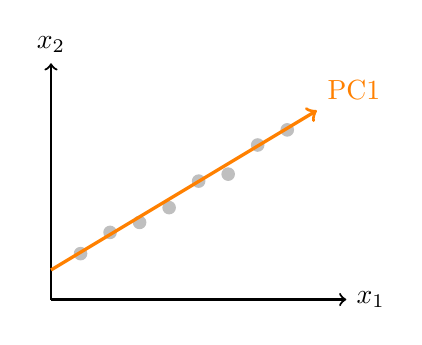
\begin{tikzpicture}[scale=0.75]
                % Fixed Axis Size for consistency
                \draw[->, thick] (0,0) -- (5,0) node[right] {$x_1$};
                \draw[->, thick] (0,0) -- (0,4) node[above] {$x_2$};
                
                % Data points roughly on a diagonal
                \foreach \x in {0.5, 1, 1.5, 2, 2.5, 3, 3.5, 4}
                    \filldraw [gray!50] (\x, 0.6*\x + 0.5 + 0.2*rand) circle (3pt);
                
                % PC1 Line
                \draw [orange, very thick, ->] (0,0.5) -- (4.5,3.2) node[above right] {PC1};
            \end{tikzpicture}
        \end{column}
    \end{columns}
\end{frame}

\begin{frame}{Types of Machine Learning}
    \begin{block}{3. Reinforcement Learning}
        Learning through trial and error. An \textbf{Agent} takes actions in an \textbf{Environment} to maximize cumulative \textbf{Reward}.
    \end{block}
    \vspace{1em}

\centering
    \begin{tikzpicture}[
        auto,
        node distance=4cm, % Increased distance for breathing room
        block/.style={
            rectangle, 
            draw, 
            text width=2.5cm, 
            text centered, 
            rounded corners, 
            minimum height=1.5cm,
            font=\large\bfseries
        },
        line/.style={draw, -{Latex[length=3mm]}, thick}
    ]
        % Nodes
        \node [block, fill=blue!10] (agent) {Agent};
        \node [block, fill=green!10, right=of agent] (env) {Environment};

        % Curved Arrows (The standard RL Loop look)
        \path [line] (agent) edge[bend left=30] node[above] {Action ($A_t$)} (env);
        \path [line] (env) edge[bend left=30] node[below] {State ($S_t$), Reward ($R_t$)} (agent);
        
    \end{tikzpicture}
    
    \vspace{1em}
    \begin{itemize}
        \item \textbf{Examples}: Chess engines (AlphaZero), Robot navigation, Stock trading bots, LLMs Preference Finetuning (RLHF).
    \end{itemize}
\end{frame}

\subsection{The Three Pillars of Learning}

\begin{frame}{The Three Pillars of Learning}
    Every supervised learning algorithm consists of three specific components
    \vspace{1em}
    \begin{enumerate}
        \item \textbf{The Hypothesis (Model)}
        \item \textbf{The Loss Function}
        \item \textbf{The Optimizer}
    \end{enumerate}
    \vspace{1em}
    
\end{frame}

\begin{frame}{1. The Hypothesis (The Model)}
    \begin{itemize}
        \item The mathematical function that maps inputs to predictions.
        \item \textbf{Notation}: $\hat{y} = f(x)$.
        \item It contains \textbf{parameters} (weights) that determine its behavior.
        \item A model is \textbf{"trained"} when these parameters are updated to fit data.
        \item It can be simple (Linear) or complex (Non-linear).
    \end{itemize}
    
    \vspace{0.5em}
    % --- Visual Examples of Models ---
    \begin{columns}[T]
        % 1. Linear Model
        \begin{column}{0.33\textwidth}
            \centering
            \small \textit{Linear Regression}\\[0.3em]
            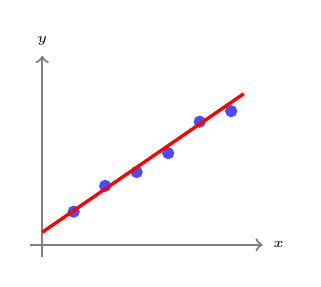
\begin{tikzpicture}[scale=0.8]
                % Axes
                \draw[->, thick, gray] (-0.2,0) -- (3.5,0) node[right, black] {\tiny $x$};
                \draw[->, thick, gray] (0,-0.2) -- (0,3) node[above, black] {\tiny $y$};
                
                % Data points
                \foreach \x in {0.5,1,1.5,2,2.5,3} 
                    \filldraw [blue!70] (\x, 0.7*\x + 0.2 + 0.2*rand) circle (2.5pt);
                
                % Regression line
                \draw [red, very thick] (0,0.2) -- (3.2,2.4);
            \end{tikzpicture}
            
            \vspace{0.3em}
            \small $\hat{y} = wx + b$
        \end{column}
        
        % 2. Decision Tree
        \begin{column}{0.33\textwidth}
            \centering
            \small \textit{Decision Tree}\\[0.3em]
            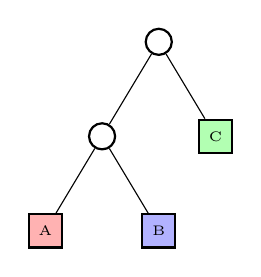
\begin{tikzpicture}[
                scale=0.8,
                level distance=1.5cm,
                sibling distance=1.8cm,
                every node/.style={font=\footnotesize}
            ]
                \node [circle, draw, thick, minimum size=8pt] {}
                    child {node [circle, draw, thick, minimum size=8pt] {}
                        child {node [rectangle, draw, thick, fill=red!30, minimum size=12pt] {\tiny A}}
                        child {node [rectangle, draw, thick, fill=blue!30, minimum size=12pt] {\tiny B}}
                    }
                    child {node [rectangle, draw, thick, fill=green!30, minimum size=12pt] {\tiny C}};
            \end{tikzpicture}
            
            \vspace{1em}
            \small $\hat{y} = \text{tree}(x)$
        \end{column}
        
        % 3. Neural Network
        \begin{column}{0.33\textwidth}
            \centering
            \small \textit{Neural Network}\\[0.3em]
            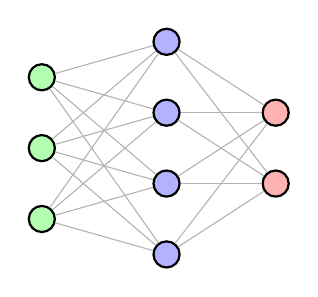
\begin{tikzpicture}[
                scale=0.9,
                x=1.1cm, y=1.0cm,
                every node/.style={circle, draw, thick, minimum size=8pt}
            ]
                % Input Layer (3 neurons)
                \node[fill=green!30] (I1) at (0,3) {};
                \node[fill=green!30] (I2) at (0,2) {};
                \node[fill=green!30] (I3) at (0,1) {};
                
                % Hidden Layer (4 neurons)
                \node[fill=blue!30] (H1) at (1.6,3.5) {};
                \node[fill=blue!30] (H2) at (1.6,2.5) {};
                \node[fill=blue!30] (H3) at (1.6,1.5) {};
                \node[fill=blue!30] (H4) at (1.6,0.5) {};
                
                % Output Layer (2 neurons)
                \node[fill=red!30] (O1) at (3,2.5) {};
                \node[fill=red!30] (O2) at (3,1.5) {};
                
                % Connections - Input to Hidden
                \foreach \i in {1,2,3}
                    \foreach \h in {1,2,3,4}
                        \draw[gray!60, line width=0.4pt] (I\i) -- (H\h);
                
                % Connections - Hidden to Output
                \foreach \h in {1,2,3,4}
                    \foreach \o in {1,2}
                        \draw[gray!60, line width=0.4pt] (H\h) -- (O\o);
            \end{tikzpicture}
            
            \vspace{0.3em}
            \small $\hat{y} = \sigma(W_2\sigma(W_1x))$
        \end{column}
    \end{columns}
\end{frame}

\begin{frame}{2. The Loss Function (The Critic)}
    \begin{columns}[T]
        % Left column: Text content
        \begin{column}{0.48\textwidth}
            \item \textbf{Definition}: A differentiable function $J(\theta)$ that quantifies the \textit{cost} of the model's errors.
            \vspace{0.5em}
            
            \textbf{Goal:} Find model parameters $\theta$ that minimize $J(\theta)$.
            
            \vspace{0.8em}
            \textbf{Common Loss Functions:}
            \begin{itemize}
                \item \textbf{\small Mean Squared Error (MSE)}\\
                (for regression tasks)
                
                \vspace{0.3em}
                \item \textbf{\small Cross-Entropy Loss (Logloss)}\\
                (for classification tasks)
            \end{itemize}
            
            \vspace{0.5em}
            \small\textit{Lower loss = Better model}
            
            \vspace{1em}
            \small{- But how can we minimize the loss?}
        \end{column}
        
        % Right column: Visualization
        \begin{column}{0.48\textwidth}
            \centering
            \textbf{Visualizing Regression Loss}
            
            \vspace{0.5em}
            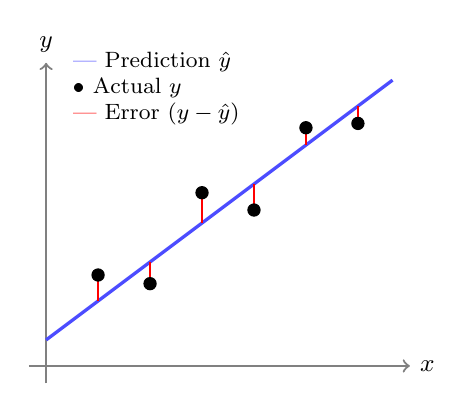
\begin{tikzpicture}[scale=1.1]
                % Axes
                \draw[->, thick, gray] (-0.2,0) -- (4.2,0) node[right, black] {\small $x$};
                \draw[->, thick, gray] (0,-0.2) -- (0,3.5) node[above, black] {\small $y$};
                
                % Regression line
                \draw [blue!70, very thick] (0,0.3) -- (4,3.3);
                
                % Data points and residuals
                \foreach \x/\offset in {0.6/0.3, 1.2/-0.25, 1.8/0.35, 2.4/-0.3, 3.0/0.2, 3.6/-0.2} {
                    \pgfmathsetmacro{\yline}{0.3 + 0.75*\x}
                    \pgfmathsetmacro{\ypoint}{\yline + \offset}
                    \pgfmathsetmacro{\absoffset}{abs(\offset)}
                    
                    % Red vertical line (residual)
                    \draw[red, thick] (\x, \yline) -- (\x, \ypoint);
                    
                    % % Red square showing squared error (correct square)
                    % \fill[red!20, opacity=0.7] (\x, \yline) rectangle ++(\absoffset, \offset);
                    % \draw[red!50, thick] (\x, \yline) rectangle ++(\absoffset, \offset);
                    
                    % Data point
                    \filldraw [black] (\x, \ypoint) circle (2pt);
                }
                
                % Legend
                \node[anchor=west, align=left, font=\footnotesize] at (0.2, 3.2) {
                    \textcolor{blue!70}{—} Prediction $\hat{y}$\\
                    \textcolor{black}{•} Actual $y$\\
                    \textcolor{red}{—} Error $(y-\hat{y})$
                };
            \end{tikzpicture}
            
            \vspace{0.5em}
            \small\textit{The loss function sums up these red distances (absolute/square).}
        \end{column}
    \end{columns}
\end{frame}

\begin{frame}{3. The Optimizer (The Teacher)}
    
    \textbf{Definition:} The algorithm that updates parameters $\theta$ to minimize loss $J(\theta)$.
    
    \vspace{1em}
    
    \begin{columns}[T]
        % --- Left: Closed Form ---
        \begin{column}{0.48\textwidth}
            \centering
            \textbf{Closed-Form Solution}
            
            \vspace{0.5em}
            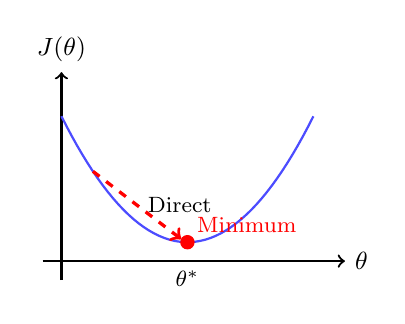
\begin{tikzpicture}[scale=0.8]
                % Axes
                \draw[->, thick] (-0.3,0) -- (4.5,0) node[right] {\small $\theta$};
                \draw[->, thick] (0,-0.3) -- (0,3) node[above] {\small $J(\theta)$};
                
                % Loss curve (parabola)
                \draw[thick, blue!70, domain=0:4, samples=50] plot (\x, {0.5*(\x-2)^2 + 0.3});
                
                % Direct arrow to minimum
                \draw[->, very thick, red, dashed] (0.5, {0.5*(0.5-2)^2 + 0.3}) -- (1.9, 0.35) node[midway, right, black] {\footnotesize Direct};
                
                % Minimum point
                \filldraw[red] (2, 0.3) circle (3pt);
                \node[below] at (2, 0) {\footnotesize $\theta^*$};
                \node[above right, red] at (2, 0.3) {\footnotesize Minimum};
            \end{tikzpicture}
            
            \vspace{0.8em}
            
            {\small 
            \textcolor{green!50!black}{\textbf{+}} Finds exact solution instantly\\
            \textcolor{red}{\textbf{$-$}} Only works for simple problems\\
            \textcolor{red}{\textbf{$-$}} Impossible for neural networks
            }
        \end{column}
        
        % --- Right: Gradient Descent ---
        \begin{column}{0.48\textwidth}
            \centering
            \textbf{Gradient Descent (Iterative)}
            
            \vspace{0.5em}
            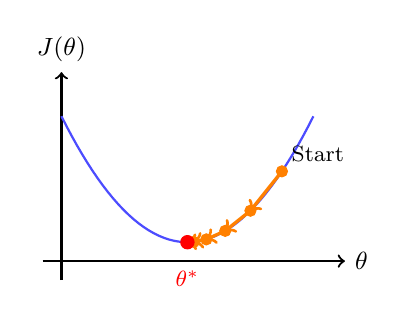
\begin{tikzpicture}[scale=0.8]
                % Axes
                \draw[->, thick] (-0.3,0) -- (4.5,0) node[right] {\small $\theta$};
                \draw[->, thick] (0,-0.3) -- (0,3) node[above] {\small $J(\theta)$};
                
                % Loss curve (parabola)
                \draw[thick, blue!70, domain=0:4, samples=50] plot (\x, {0.5*(\x-2)^2 + 0.3});
                
                % Iterative steps - calculated to be on the curve y = 0.5*(x-2)^2 + 0.3
                \coordinate (p0) at (3.5, {0.5*(3.5-2)^2 + 0.3});
                \coordinate (p1) at (3.0, {0.5*(3.0-2)^2 + 0.3});
                \coordinate (p2) at (2.6, {0.5*(2.6-2)^2 + 0.3});
                \coordinate (p3) at (2.3, {0.5*(2.3-2)^2 + 0.3});
                \coordinate (p4) at (2.1, {0.5*(2.1-2)^2 + 0.3});
                \coordinate (p5) at (2.0, {0.5*(2.0-2)^2 + 0.3});
                
                \filldraw[orange] (p0) circle (2.5pt);
                \draw[->, very thick, orange] (p0) -- (p1);
                \filldraw[orange] (p1) circle (2.5pt);
                \draw[->, very thick, orange] (p1) -- (p2);
                \filldraw[orange] (p2) circle (2.5pt);
                \draw[->, very thick, orange] (p2) -- (p3);
                \filldraw[orange] (p3) circle (2.5pt);
                \draw[->, very thick, orange] (p3) -- (p4);
                \filldraw[orange] (p4) circle (2.5pt);
                \draw[->, very thick, orange] (p4) -- (p5);
                \filldraw[red] (p5) circle (3pt);
                
                % Label
                \node[above right, black] at (p0) {\footnotesize Start};
                \node[below, red] at (2, 0) {\footnotesize $\theta^*$};
            \end{tikzpicture}
            
            \vspace{0.8em}
            
            {\small 
            \textcolor{green!50!black}{\textbf{+}} Works for any model\\
            \textcolor{green!50!black}{\textbf{+}} Universal for ML/DL\\
            \textcolor{orange!80!black}{\textbf{$-$}} Requires many iterations
            }
        \end{column}
    \end{columns}
    
    % \vspace{1em}
    % \centering
    % \small\textit{Update rule: } $\theta_{new} = \theta_{old} - \alpha \nabla J(\theta)$ \quad {\footnotesize($\alpha$ = learning rate)}
    
\end{frame}





\begin{frame}{How Gradient Descent Works}
    
    \textbf{Core Idea:} Move parameters in the direction that reduces loss.
    
    \vspace{1em}
    
    \begin{columns}[c]
        % Left: Visual
        \begin{column}{0.45\textwidth}
            \centering
            \begin{tikzpicture}[scale=1.1]
                % Axes
                \draw[->, thick] (-0.3,0) -- (4.5,0) node[right] {\small $\theta$};
                \draw[->, thick] (0,-0.3) -- (0,3.2) node[above] {\small $J(\theta)$};
                
                % Loss curve
                \draw[thick, blue!70, domain=0:4, samples=50] plot (\x, {0.5*(\x-2)^2 + 0.3});
                
                % Current point
                \coordinate (current) at (3.2, {0.5*(3.2-2)^2 + 0.3});
                \filldraw[black!80, fill=black!60] (current) circle (3.5pt);
                \node[right=3pt, black!80] at (current) {$\theta_t$};
                
                % % Tangent line (gradient)
                % \draw[orange, very thick, <->] (2.7, 1.1) -- (3.7, 1.9);
                % \node[above, orange] at (3.2, 1.7) {\footnotesize Slope = $\nabla J(\theta_t)$};
                
                % Arrow showing update direction
                \draw[->, !60!black, line width=2pt]
                (current) -- ++(-0.6, -0.5)
                node[left=15pt, above=8pt, font=\footnotesize] {$-\alpha \nabla J$};

                
                % Next point
                \coordinate (next) at (2.5, {0.5*(2.5-2)^2 + 0.3});
                \filldraw[red!60!black, fill=red!40] (next) circle (3.5pt);
                \node[below, red!60!black] at (next) {$\theta_{t+1}$};
            \end{tikzpicture}
        \end{column}
        
        % Right: Steps
        \begin{column}{0.5\textwidth}
            \textbf{Step-by-Step Process:}
            
            \vspace{0.5em}
            
            \begin{enumerate}
                \item \textbf{Compute Loss}\\
                {\small Evaluate $J(\theta_t)$ at current parameters}
                
                \vspace{0.3em}
                
                \item \textbf{Calculate Gradient}\\
                {\small Find slope: $\nabla J(\theta_t) = \frac{\partial J}{\partial \theta}$}
                
                \vspace{0.3em}
                
                \item \textbf{Update Parameters}\\
                {\small Move opposite to gradient with a step size (learning rate) $\alpha$:}
                $$\theta_{t+1} = \theta_t - \alpha \nabla J(\theta_t)$$
                
                % \vspace{0.3em}
                
                \item \textbf{Repeat}\\
                {\small Until convergence (loss stops decreasing)}
            \end{enumerate}

        \end{column}
    \end{columns}
    
\end{frame}


\subsection{The Learning Loop}

\begin{frame}{Putting It All Together: The Learning Loop}
    \centering
    
    \vspace{0.25em}
    
    \begin{tikzpicture}[
        node distance=2.0cm,
        auto,
        thick,
        % Styles for the blocks
        block/.style={
            rectangle, 
            draw, 
            rounded corners=5pt,
            text width=2.4cm, 
            text centered, 
            minimum height=1.1cm,
            font=\small\bfseries,
            line width=1.1pt
        },
        line/.style={draw, -{Latex[length=2.3mm]}, line width=1.1pt}
    ]
        % --- Nodes ---
        % 1. Data (left)
        \node [block, fill=gray!20] (data) {Data\\$(x, y)$};
        
        % 2. Model (center)
        \node [block, fill=blue!20, right=1.3cm of data] (model) {Model\\$\hat{y} = f_\theta(x)$};
        
        % 3. Loss (right)
        \node [block, fill=red!20, right=1.9cm of model] (loss) {Loss Function\\$J(\theta)$};
        
        % 4. Optimizer (below model)
        \node [block, fill=green!20, below=1.0cm of model] (opt) {Optimizer};
        
        % --- Flows ---
        % Data -> Model (input x)
        \path [line, blue!70] (data) -- node [below, black] {\scriptsize Input $x$} (model);
        
        % Data -> Loss (true labels y)
        \path [line, gray!70] (data.north) to[bend left=15] node [above, black, pos=0.5] {\scriptsize True $y$} (loss.north);
        
        % Model -> Loss (predictions)
        \path [line, red!70] (model) -- node [below, black] {\scriptsize Predictions $\hat{y}$} (loss);
        
        % Loss -> Optimizer (gradients)
        \path [line, orange!70] (loss.south) to[bend left=20] node [left, black, pos=0.3] {\scriptsize Compute $\nabla J$} (opt.east);
        
        % Optimizer -> Model (update weights)
        \path [line, green!70] (opt) -- node [left, black] {\scriptsize Update $\theta$} (model);
        
    \end{tikzpicture}
    
    \vspace{0.5em}
    
    \begin{columns}[T]
        \begin{column}{0.48\textwidth}
            \textbf{Forward Pass:}
            \begin{itemize}
                \item Data $\to$ Model $\to$ Predictions
                \item Compute Loss
            \end{itemize}
        \end{column}
        
        \begin{column}{0.48\textwidth}
            \textbf{Backward Pass:}
            \begin{itemize}
                \item Calculate gradients
                \item Update parameters
            \end{itemize}
        \end{column}
    \end{columns}
    
    \vspace{0.25em}
    \centering
    \textit{Repeat until loss converges (model learns)!}
    
\end{frame}








% =========================
% 3. Main Challenges
% =========================

\section{Main Challenges of Machine Learning}

\begin{frame}{What Can Go Wrong?}
    Since our task is to select a learning algorithm and train it on data, there are two main sources of failure:
    \vspace{1em}
    \begin{columns}[c]
        \begin{column}{0.50\textwidth}
            \centering
            \begin{tcolorbox}[colback=red!5, colframe=red!60, title=\textbf{1. Bad Data}]
                \begin{itemize}
                    \item Not enough data
                    \item Non-representative data
                    \item Poor quality (Noise)
                    \item Irrelevant features
                \end{itemize}
            \end{tcolorbox}
        \end{column}
        \begin{column}{0.03\textwidth}
            \centering \textbf{+}
        \end{column}
        \begin{column}{0.52\textwidth}
            \centering
            \begin{tcolorbox}[colback=blue!5, colframe=blue!60, title=\textbf{2. Bad Algorithm}]
                \begin{itemize}
                    \item Overfitting
                    \item Underfitting
                \end{itemize}
            \end{tcolorbox}
        \end{column}
    \end{columns}
\end{frame}


% --- SLIDE 1: INSUFFICIENT DATA (The Scale Plot) ---
\begin{frame}{Problem 1: Insufficient Data}

    \begin{columns}[c]
        \begin{column}{0.4\textwidth}
            \textbf{The Reality Gap}
            \vspace{1em}
            \begin{itemize}
                \item \textbf{Humans:} Can generalize from 1 example (Zero-shot).
                \item \textbf{Machines:} Need thousands to find the signal in the noise.
            \end{itemize}
            
            \vspace{1em}
            \small \textit{Without enough data, complex models just memorize the noise.}
        \end{column}

        \begin{column}{0.6\textwidth}
            \centering
            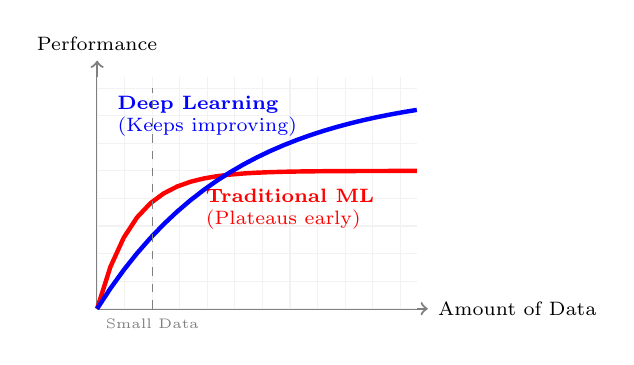
\begin{tikzpicture}[scale=0.7]
                % Axes
                \draw[->, thick, gray] (0,0) -- (6,0) node[right, black] {\scriptsize Amount of Data};
                \draw[->, thick, gray] (0,0) -- (0,4.5) node[above, black] {\scriptsize Performance};
                
                % Grid
                \draw[gray!10, step=0.5] (0,0) grid (5.8,4.2);

                % Traditional ML (Plateau)
                \draw[red, ultra thick, domain=0:5.8] plot (\x, {2.5 * (1 - exp(-1.5*\x))});
                \node[red, align=left, font=\scriptsize] at (3.5, 1.8) {\textbf{Traditional ML}\\(Plateaus early)};
                
                % Deep Learning (Scale)
                \draw[blue, ultra thick, domain=0:5.8] plot (\x, {4.0 * (1 - exp(-0.4*\x))});
                \node[blue, align=left, font=\scriptsize] at (2.0, 3.5) {\textbf{Deep Learning}\\(Keeps improving)};
                
                % Dotted connector
                \draw[dashed, gray] (1, 0) -- (1, 4);
                \node[below, font=\tiny, gray] at (1,0) {Small Data};
            \end{tikzpicture}
        \end{column}
    \end{columns}
\end{frame}

% --- SLIDE 2: SAMPLING BIAS (Text Only) ---
\begin{frame}{Problem 2: Non-Representative Data (Bias)}

    \begin{alertblock}{Definition: Sampling Bias}
        When your training data does not accurately reflect the real world you want to predict.
    \end{alertblock}


    \begin{tcolorbox}[colback=blue!5, colframe=blue!50, title=Example: The "Happiness" Model]
        \textbf{Scenario:}
        \begin{itemize}
            \item You want to predict \textbf{Happiness} based on \textbf{Wealth}.
            \item But you only collect data from the \textbf{Middle Class}.
        \end{itemize}
        
        \vspace{0.5em}
        \textbf{The Result:}
        \begin{itemize}
            \item The model learns: \textit{"More Money = More Happy."}
            \item \textbf{Fail:} It will fail catastrophically for \textbf{Billionaires} (where money stops mattering) or \textbf{Poverty} (where struggles are different).
        \end{itemize}
    \end{tcolorbox}

\end{frame}

\begin{frame}{Problems 3 \& 4: Poor Quality \& Irrelevant Features}
    \begin{columns}[T]
        \begin{column}{0.48\textwidth}
            \textbf{Poor Quality Data}
            \begin{itemize}
                \item \textbf{Noise:} Random errors in the data.
                \item \textbf{Outliers:} Extreme values that distort the pattern.
                \item \textbf{Missing Values:} Empty cells in your spreadsheet.
            \end{itemize}
            \vspace{0.5em}
            \textit{Solution: Data Cleaning (takes ~80\% of a Data Scientist's time).}
        \end{column}
        \begin{column}{0.48\textwidth}
            \textbf{Irrelevant Features}
            \begin{itemize}
                \item \textit{"Garbage In, Garbage Out"}
                \item If you try to predict "Price of a Car" using "Color of the seats", the model will fail.
            \end{itemize}
            \vspace{0.5em}
            \textit{Solution: Feature Engineering (Selection \& Extraction).}
        \end{column}
    \end{columns}
\end{frame}

% --- Subsection: Bad Algorithm ---
\section{Generalization}
\subsection{Overfitting vs. Underfitting}
\begin{frame}{Algorithm Problem: Generalization}
    \centering
    \begin{columns}[T]
        % --- Column 1: Simple fit ---
        \begin{column}{0.32\textwidth}
            \centering
            \textbf{\small Model A}\\[0.3em]
            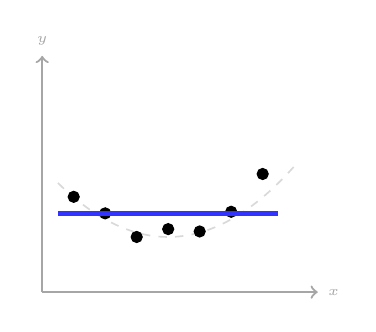
\begin{tikzpicture}[scale=1.0]
                % Axes
                \draw[->, thick, gray!70] (0,0) -- (3.5,0) node[right] {\tiny $x$};
                \draw[->, thick, gray!70] (0,0) -- (0,3) node[above] {\tiny $y$};
                % True curve (hidden to the model, just our reference)
                \draw[gray!30, dashed, line width=0.6pt, domain=0.2:3.2, samples=50] 
                    plot (\x, {0.35*(\x-1.6)^2 + 0.7});
                % Training data points
                \foreach \x/\y in {0.4/1.21, 0.8/1.0, 1.2/0.70, 1.6/0.80, 2.0/0.77, 2.4/1.02, 2.8/1.5}
                    \filldraw[black] (\x,\y) circle (2pt);
                % Simple model: flat line
                \draw[blue!80, line width=2pt] (0.2,1.0) -- (3.0,1.0);
            \end{tikzpicture}
            \vspace{0.3em}
            {\footnotesize Train MSE $\approx 0.20$}
        \end{column}
        
        % --- Column 2: Reasonable fit ---
        \begin{column}{0.32\textwidth}
            \centering
            \textbf{\small Model B}\\[0.3em]
            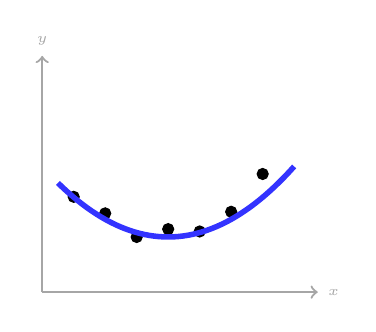
\begin{tikzpicture}[scale=1.0]
                % Axes
                \draw[->, thick, gray!70] (0,0) -- (3.5,0) node[right] {\tiny $x$};
                \draw[->, thick, gray!70] (0,0) -- (0,3) node[above] {\tiny $y$};
                % Training data points
                \foreach \x/\y in {0.4/1.21, 0.8/1.0, 1.2/0.70, 1.6/0.80, 2.0/0.77, 2.4/1.02, 2.8/1.5}
                    \filldraw[black] (\x,\y) circle (2pt);
                % Smooth curve through the trend
                \draw[blue!80, line width=2pt, domain=0.2:3.2, samples=50] 
                    plot (\x, {0.35*(\x-1.6)^2 + 0.7});
            \end{tikzpicture}
            \vspace{0.3em}
            {\footnotesize Train MSE $\approx 0.06$}
        \end{column}
        
        % --- Column 3: Very wiggly fit ---
        \begin{column}{0.32\textwidth}
            \centering
            \textbf{\small Model C}\\[0.3em]
            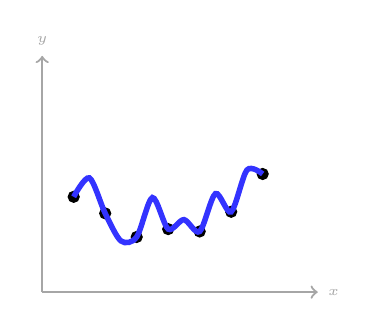
\begin{tikzpicture}[scale=1.0]
                % Axes
                \draw[->, thick, gray!70] (0,0) -- (3.5,0) node[right] {\tiny $x$};
                \draw[->, thick, gray!70] (0,0) -- (0,3) node[above] {\tiny $y$};
                % Training data points
                \foreach \x/\y in {0.4/1.21, 0.8/1.0, 1.2/0.70, 1.6/0.80, 2.0/0.77, 2.4/1.02, 2.8/1.5}
                    \filldraw[black] (\x,\y) circle (2pt);
                % Wiggly curve going exactly through points
                \draw[blue!80, line width=2pt, smooth] 
                    plot coordinates {
                        (0.4,1.21) (0.6,1.45) (0.8,1.0) (1.0,0.65) 
                        (1.2,0.70) (1.4,1.2) (1.6,0.8) (1.8,0.92) 
                        (2.0,0.77) (2.2,1.25) (2.4,1.02) (2.6,1.55) (2.8,1.5)
                    };
            \end{tikzpicture}
            \vspace{0.3em}
            {\footnotesize Train MSE $\approx 0.00$}
        \end{column}
    \end{columns}
    
    \vspace{0.6em}
    \centering
    \small
    All three models see the same training points but fit them in very different ways.  
    Which one should we pick?
\end{frame}

\begin{frame}{What Do We Really Want?}
    \begin{itemize}
        \item We care about how the model behaves on \textbf{new unseen data}, not only on the points it has already seen
        \item Imagine we now collect a few fresh samples from the same process
    \end{itemize}
    
    \vspace{0.6em}
    \centering
    \begin{columns}[T]
        % --- Column 1: Model A with new points ---
        \begin{column}{0.32\textwidth}
            \centering
            \textbf{\small Model A}\\[0.3em]
            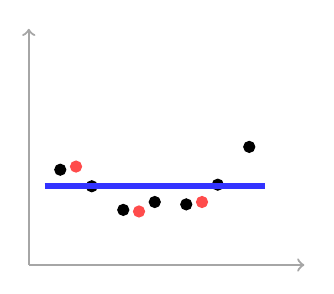
\begin{tikzpicture}[scale=1.0]
                % Axes
                \draw[->, thick, gray!70] (0,0) -- (3.5,0);
                \draw[->, thick, gray!70] (0,0) -- (0,3);
                % Training data
                \foreach \x/\y in {0.4/1.21, 0.8/1.0, 1.2/0.70, 1.6/0.80, 2.0/0.77, 2.4/1.02, 2.8/1.5}
                    \filldraw[black] (\x,\y) circle (2pt);
                % New data points (e.g. test)
                \foreach \x/\y in {0.6/1.25, 1.4/0.68, 2.2/0.8}
                    \filldraw[red!70] (\x,\y) circle (2pt);
                % Simple model
                \draw[blue!80, line width=2pt] (0.2,1.0) -- (3.0,1.0);
            \end{tikzpicture}
        \end{column}
        
        % --- Column 2: Model B with new points ---
        \begin{column}{0.32\textwidth}
            \centering
            \textbf{\small Model B}\\[0.3em]
            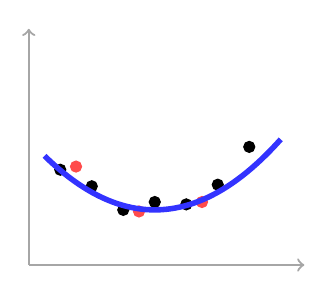
\begin{tikzpicture}[scale=1.0]
                % Axes
                \draw[->, thick, gray!70] (0,0) -- (3.5,0);
                \draw[->, thick, gray!70] (0,0) -- (0,3);
                % Training data
                \foreach \x/\y in {0.4/1.21, 0.8/1.0, 1.2/0.70, 1.6/0.80, 2.0/0.77, 2.4/1.02, 2.8/1.5}
                    \filldraw[black] (\x,\y) circle (2pt);
                % New data
                \foreach \x/\y in {0.6/1.25, 1.4/0.68, 2.2/0.8}
                    \filldraw[red!70] (\x,\y) circle (2pt);
                % Smooth curve
                \draw[blue!80, line width=2pt, domain=0.2:3.2, samples=50] 
                    plot (\x, {0.35*(\x-1.6)^2 + 0.7});
            \end{tikzpicture}
        \end{column}
        
        % --- Column 3: Model C with new points ---
        \begin{column}{0.32\textwidth}
            \centering
            \textbf{\small Model C}\\[0.3em]
            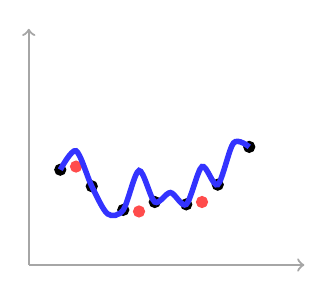
\begin{tikzpicture}[scale=1.0]
                % Axes
                \draw[->, thick, gray!70] (0,0) -- (3.5,0);
                \draw[->, thick, gray!70] (0,0) -- (0,3);
                % Training data
                \foreach \x/\y in {0.4/1.21, 0.8/1.0, 1.2/0.70, 1.6/0.80, 2.0/0.77, 2.4/1.02, 2.8/1.5}
                    \filldraw[black] (\x,\y) circle (2pt);
                % New data
                \foreach \x/\y in {0.6/1.25, 1.4/0.68, 2.2/0.8}
                    \filldraw[red!70] (\x,\y) circle (2pt);
                % Wiggly curve
                \draw[blue!80, line width=2pt, smooth] 
                    plot coordinates {
                        (0.4,1.21) (0.6,1.45) (0.8,1.0) (1.0,0.65) 
                        (1.2,0.70) (1.4,1.2) (1.6,0.8) (1.8,0.92) 
                        (2.0,0.77) (2.2,1.25) (2.4,1.02) (2.6,1.55) (2.8,1.5)
                    };
            \end{tikzpicture}
        \end{column}
    \end{columns}
    
    \vspace{0.5em}
    \small
    On these new red points, Model B stays close, while Model A and Model C miss more.  
\end{frame}

\begin{frame}{Underfit vs Good Fit vs Overfit}
    \centering
    \begin{columns}[T]
        % --- Column 1: Underfit ---
        \begin{column}{0.32\textwidth}
            \centering
            \textbf{\small Underfit}\\[0.3em]
            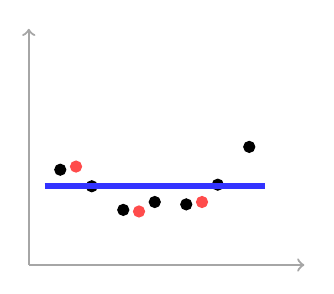
\begin{tikzpicture}[scale=1.0]
                \draw[->, thick, gray!70] (0,0) -- (3.5,0);
                \draw[->, thick, gray!70] (0,0) -- (0,3);
                % Train data
                \foreach \x/\y in {0.4/1.21, 0.8/1.0, 1.2/0.70, 1.6/0.80, 2.0/0.77, 2.4/1.02, 2.8/1.5}
                    \filldraw[black] (\x,\y) circle (2pt);
                % New data
                \foreach \x/\y in {0.6/1.25, 1.4/0.68, 2.2/0.8}
                    \filldraw[red!70] (\x,\y) circle (2pt);
                % Simple model
                \draw[blue!80, line width=2pt] (0.2,1.0) -- (3.0,1.0);
            \end{tikzpicture}
            \vspace{0.4em}
            \begin{tcolorbox}[colback=red!5, colframe=red!40, boxrule=0.5pt, arc=2mm, left=2pt, right=2pt, top=2pt, bottom=2pt]
                \centering \small \textbf{Too Simple\\(High Bias)}\\Ignores patterns
            \end{tcolorbox}
        \end{column}
        
        % --- Column 2: Good Fit ---
        \begin{column}{0.32\textwidth}
            \centering
            \textbf{\small Good Fit}\\[0.3em]
            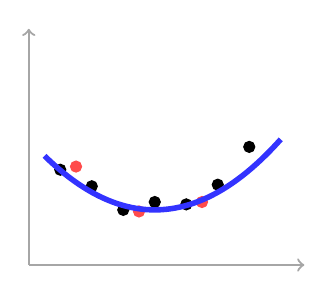
\begin{tikzpicture}[scale=1.0]
                \draw[->, thick, gray!70] (0,0) -- (3.5,0);
                \draw[->, thick, gray!70] (0,0) -- (0,3);
                % Train data
                \foreach \x/\y in {0.4/1.21, 0.8/1.0, 1.2/0.70, 1.6/0.80, 2.0/0.77, 2.4/1.02, 2.8/1.5}
                    \filldraw[black] (\x,\y) circle (2pt);
                % New data
                \foreach \x/\y in {0.6/1.25, 1.4/0.68, 2.2/0.8}
                    \filldraw[red!70] (\x,\y) circle (2pt);
                % Reasonable curve
                \draw[blue!80, line width=2pt, domain=0.2:3.2, samples=50] 
                    plot (\x, {0.35*(\x-1.6)^2 + 0.7});
            \end{tikzpicture}
            \vspace{0.4em}
            \begin{tcolorbox}[colback=green!5, colframe=black!40, boxrule=0.5pt, arc=2mm, left=2pt, right=2pt, top=2pt, bottom=2pt]
                \centering \small \textbf{Captures Structure}\\Balanced
            \end{tcolorbox}
        \end{column}
        
        % --- Column 3: Overfit ---
        \begin{column}{0.32\textwidth}
            \centering
            \textbf{\small Overfit}\\[0.3em]
            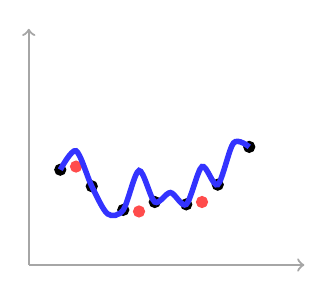
\begin{tikzpicture}[scale=1.0]
                \draw[->, thick, gray!70] (0,0) -- (3.5,0);
                \draw[->, thick, gray!70] (0,0) -- (0,3);
                % Train data
                \foreach \x/\y in {0.4/1.21, 0.8/1.0, 1.2/0.70, 1.6/0.80, 2.0/0.77, 2.4/1.02, 2.8/1.5}
                    \filldraw[black] (\x,\y) circle (2pt);
                % New data
                \foreach \x/\y in {0.6/1.25, 1.4/0.68, 2.2/0.8}
                    \filldraw[red!70] (\x,\y) circle (2pt);
                % Wiggly curve
                \draw[blue!80, line width=2pt, smooth] 
                    plot coordinates {
                        (0.4,1.21) (0.6,1.45) (0.8,1.0) (1.0,0.65) 
                        (1.2,0.70) (1.4,1.2) (1.6,0.8) (1.8,0.92) 
                        (2.0,0.77) (2.2,1.25) (2.4,1.02) (2.6,1.55) (2.8,1.5)
                    };
            \end{tikzpicture}
            \vspace{0.4em}
            \begin{tcolorbox}[colback=red!5, colframe=red!40, boxrule=0.5pt, arc=2mm, left=2pt, right=2pt, top=2pt, bottom=2pt]
                \centering \small \textbf{Too Complex\\(High Variance)}\\Memorizes noise
            \end{tcolorbox}
        \end{column}
    \end{columns}
\end{frame}

\begin{frame}{Underfit vs Good Fit vs Overfit}
    \begin{itemize}
        \item \textbf{Underfitting}
        \begin{itemize}
            \item Model is too simple for the true pattern
            \item It cannot reach low error even with a lot of data
        \end{itemize}
        \item \textbf{Overfitting}
        \begin{itemize}
            \item Model is too flexible and learns noise
            \item It fits training points very well but is unstable on new points
        \end{itemize}
        \item \textbf{Good fit}
        \begin{itemize}
            \item Model has just enough flexibility to capture useful structure
            \item It behaves similarly on seen and unseen data
        \end{itemize}
    \end{itemize}
\end{frame}

\begin{frame}{What is Generalization?}

    \begin{block}{Definition}
        Generalization is the ability of a model to perform well on data it has \textbf{never seen before}.
    \end{block}
    
    \vspace{1em}
    
    \textbf{High Training Accuracy $\neq$ Learning}
    \begin{itemize}
        \item \textbf{Memorization (Capacity):} Modern models are powerful enough to memorize the entire training set, acting like a "lookup table" rather than a learner.
        \item \textbf{Shortcuts (Laziness):} If a simple noise pattern correlates with the target, the model will learn that instead of the complex true signal.
    \end{itemize}

\end{frame}


\begin{frame}{Examples:}
    \centering
    \small    
    \begin{table}[]
        \centering
        \renewcommand{\arraystretch}{1.4} 
        \begin{tabular}{l p{4.0cm} p{4.5cm}}
            \hline
            \textbf{Domain} & \textbf{Intended Pattern} & \textbf{Reality} \\ \hline
            \textbf{Vision} & Recognizes animal features (ears, snout). & Learns that \textbf{snow background} = Wolf. \\ 
            \textbf{Tabular} & Evaluates financial history (income, debt). & Learns that \textbf{Application Font/ID} = High Risk. \\ 
            \textbf{NLP} & Analyzes sentence semantics and sentiment. & Memorizes specific \textbf{names} (e.g., "Ali"). \\ 
            \textbf{RL} & Learns strategy to win the game/level. & Finds a \textbf{glitch} or loops indefinitely to farm points. \\ \hline
        \end{tabular}
    \end{table}
\end{frame}


\begin{frame}{Addressing Overfitting}
    \centering
    \large \textit{Since we cannot trust the training error, we need a systematic approach to validate our models.}
    
    \vspace{0.8cm}
    
    \begin{columns}[T]
        \begin{column}{0.3\textwidth}
            \begin{block}{\centering1. Detect:}
                \centering
                \textbf{Splitting Data}\\
                (Holdout, K-Fold)
            \end{block}
        \end{column}
        \begin{column}{0.3\textwidth}
            \begin{block}{\centering2. Measure:}
                \centering
                \textbf{Metrics}\\
                (Accuracy, MSE, F1, AUC)
            \end{block}
        \end{column}
        \begin{column}{0.3\textwidth}
            \begin{block}{\centering3. Mitigate:}
                \centering
                \textbf{Strategies}\\
                (Regularization, More Data, Better Features)
            \end{block}
        \end{column}
    \end{columns}
\end{frame}

\subsection{Data Splitting}

\begin{frame}{Addressing Overfitting}
    \centering
    \large \textit{Since we cannot trust the training error, we need a systematic approach to validate our models.}
    
    \vspace{0.8cm}
    
    \begin{columns}[T]
        \begin{column}{0.3\textwidth}
            \begin{block}{\centering1. Detect:}
                \centering
                \textbf{Splitting Data}\\
                (Holdout, K-Fold)
            \end{block}
        \end{column}
        \begin{column}{0.3\textwidth}
            \begin{block}{\centering2. Measure:}
                \centering
                \textbf{Metrics}\\
                (Accuracy, MSE, F1, AUC)
            \end{block}
        \end{column}
        \begin{column}{0.3\textwidth}
            \begin{block}{\centering3. Mitigate:}
                \centering
                \textbf{Strategies}\\
                (Regularization, More Data, Better Features)
            \end{block}
        \end{column}
    \end{columns}
    
    \vspace{0.5cm}
    \centering
    \small $\rightarrow$ \textit{Step 1: How to simulate "unseen data" using Splits.}
\end{frame}



\begin{frame}{Detecting Overfitting: The Holdout Split}
    \begin{itemize}
        \item We cannot trust performance on training data (memorization).
        \item \textbf{Solution:} Hide a piece of data to simulate the "Future."
    \end{itemize}
    
    \vspace{1em} % Increased vertical space before diagram
    \centering
    
    % Adjusted scale and width (0 to 12 instead of 0 to 10)
    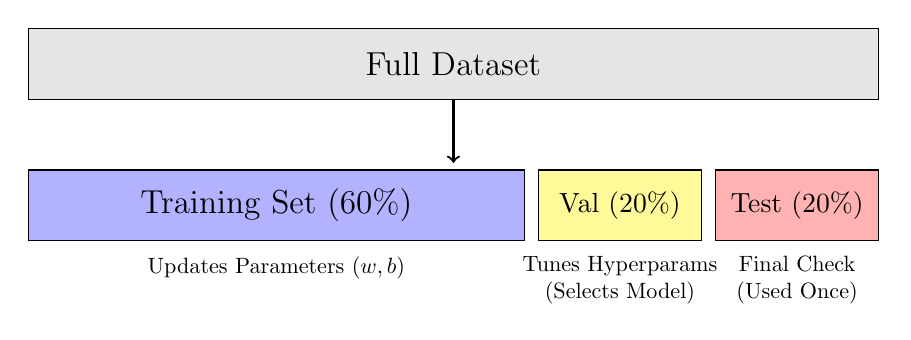
\begin{tikzpicture}[scale=0.9]
    
         % --- Full Data (Top) ---
         % Stretched width to 12, moved up to y=1.5
         \draw[fill=gray!20] (0,1.5) rectangle (12,2.5);
         \node at (6,2.0) {\large Full Dataset};
         
         % Arrow (Longer now)
         \draw[->, thick] (6,1.5) -- (6,0.6);
         
         % --- Splits (Bottom) ---
         
         % 1. Training Set (Widen to 7 units)
         \draw[fill=blue!30] (0,-0.5) rectangle (7,0.5);
         \node at (3.5,0) {\large Training Set (60\%)};
         % Text below with fixed width for cleaner wrapping
         \node[below=1mm, align=center, text width=6cm, scale=0.8] at (3.5,-0.5) 
              {Updates Parameters ($w, b$)};
         
         % 2. Validation Set (Widen to 2.3 units)
         \draw[fill=yellow!40] (7.2,-0.5) rectangle (9.5,0.5);
         \node at (8.35,0) {Val (20\%)};
         \node[below=1mm, align=center, text width=3.5cm, scale=0.8] at (8.35,-0.5) 
              {Tunes Hyperparams\\(Selects Model)};
         
         % 3. Test Set (Widen to 2.3 units)
         \draw[fill=red!30] (9.7,-0.5) rectangle (12,0.5);
         \node at (10.85,0) {Test (20\%)};
         \node[below=1mm, align=center, text width=2.5cm, scale=0.8] at (10.85,-0.5) 
              {Final Check\\(Used Once)};
              
    \end{tikzpicture}
\end{frame}

\begin{frame}{Diagnosis: Loss Curves}
    \vspace{0.5em}
    \centering
    \begin{columns}[T]
        % Column 1: Underfit
        \begin{column}{0.32\textwidth}
            \centering
            \colorbox{gray!10}{\parbox{1.05\textwidth}{
                \centering
                \vspace{0.3em}
                \textbf{\large Underfitting}\\[0.4em]
                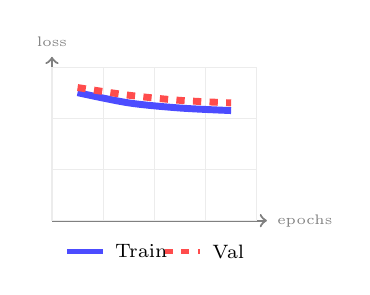
\begin{tikzpicture}[scale=0.65]
                    \draw[->, thick, gray] (0,0) -- (4.2,0) node[right, font=\tiny] {epochs};
                    \draw[->, thick, gray] (0,0) -- (0,3.2) node[above, font=\tiny] {loss};
                    \draw[gray!15, thin] (0,0) grid (4,3);
                    
                    % Train
                    \draw[blue!70, line width=2.5pt] plot[smooth] coordinates {(0.5,2.5) (1.5,2.3) (2.5,2.2) (3.5,2.15)};
                    % Val
                    \draw[red!70, line width=2.5pt, dashed] plot[smooth] coordinates {(0.5,2.6) (1.5,2.45) (2.5,2.35) (3.5,2.3)};
                    
                    % Legend
                    \draw[blue!70, line width=2pt] (0.3,-0.6) -- (1,-0.6) node[right, font=\scriptsize, black] {Train};
                    \draw[red!70, line width=2pt, dashed] (2.2,-0.6) -- (2.9,-0.6) node[right, font=\scriptsize, black] {Val};
                \end{tikzpicture}\\[0.5em]
                {\small Both losses remain \textbf{high}}\\
                {\scriptsize\color{gray} Model too simple}\\[0.3em]
            }}
        \end{column}
        
        % Column 2: Good Fit
        \begin{column}{0.32\textwidth}
            \centering
            \colorbox{green!8}{\parbox{1.05\textwidth}{
                \centering
                \vspace{0.3em}
                \textbf{\large Good Fit}\\[0.4em]
                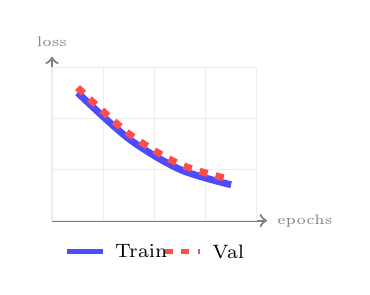
\begin{tikzpicture}[scale=0.65]
                    \draw[->, thick, gray] (0,0) -- (4.2,0) node[right, font=\tiny] {epochs};
                    \draw[->, thick, gray] (0,0) -- (0,3.2) node[above, font=\tiny] {loss};
                    \draw[gray!15, thin] (0,0) grid (4,3);
                    
                    % Train
                    \draw[blue!70, line width=2.5pt] plot[smooth] coordinates {(0.5,2.5) (1.5,1.6) (2.5,1.0) (3.5,0.7)};
                    % Val
                    \draw[red!70, line width=2.5pt, dashed] plot[smooth] coordinates {(0.5,2.6) (1.5,1.7) (2.5,1.1) (3.5,0.8)};
                    
                    % Legend
                    \draw[blue!70, line width=2pt] (0.3,-0.6) -- (1,-0.6) node[right, font=\scriptsize, black] {Train};
                    \draw[red!70, line width=2pt, dashed] (2.2,-0.6) -- (2.9,-0.6) node[right, font=\scriptsize, black] {Val};
                \end{tikzpicture}\\[0.5em]
                {\small Both losses are \textbf{low}}\\
                {\scriptsize\color{gray} Curves track down closely}\\[0.3em]
            }}
        \end{column}
        
        % Column 3: Overfit
        \begin{column}{0.32\textwidth}
            \centering
            \colorbox{orange!10}{\parbox{1.05\textwidth}{
                \centering
                \vspace{0.3em}
                \textbf{\large Overfitting}\\[0.4em]
                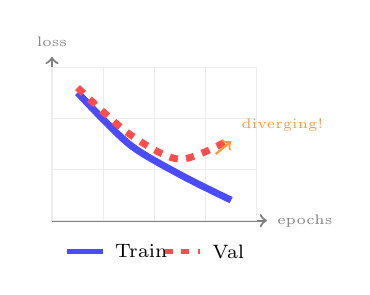
\begin{tikzpicture}[scale=0.65]
                    \draw[->, thick, gray] (0,0) -- (4.2,0) node[right, font=\tiny] {epochs};
                    \draw[->, thick, gray] (0,0) -- (0,3.2) node[above, font=\tiny] {loss};
                    \draw[gray!15, thin] (0,0) grid (4,3);
                    
                    % Train
                    \draw[blue!70, line width=2.5pt] plot[smooth] coordinates {(0.5,2.5) (1.5,1.5) (2.5,0.9) (3.5,0.4)};
                    % Val
                    \draw[red!70, line width=2.5pt, dashed] plot[smooth] coordinates {(0.5,2.6) (1.5,1.7) (2.5,1.2) (3.5,1.6)};
                    
                    % Annotation arrow
                    \draw[->, orange!80, thick] (3.2,1.3) -- (3.5,1.55) node[above right, font=\tiny] {diverging!};
                    
                    % Legend
                    \draw[blue!70, line width=2pt] (0.3,-0.6) -- (1,-0.6) node[right, font=\scriptsize, black] {Train};
                    \draw[red!70, line width=2pt, dashed] (2.2,-0.6) -- (2.9,-0.6) node[right, font=\scriptsize, black] {Val};
                \end{tikzpicture}\\[0.5em]
                {\small Train loss ↓, Val loss ↑}\\
                {\scriptsize\color{gray} Model started to overfit!}\\[0.3em]
            }}
        \end{column}
    \end{columns}
    
    \vspace{1em}
    \begin{center}
        \small\textit{The gap between training and validation loss reveals overfitting!}
    \end{center}
\end{frame}

\begin{frame}{Detecting Overfitting: The Holdout Split}
    
    \centering
    
    % Adjusted scale and width (0 to 12 instead of 0 to 10)
    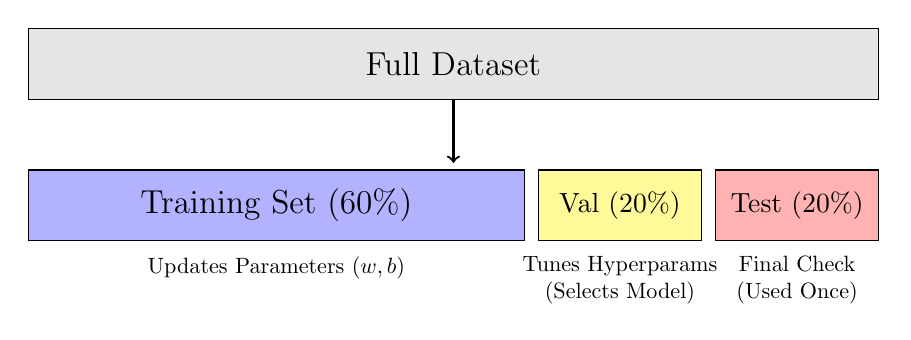
\begin{tikzpicture}[scale=0.9]
    
         % --- Full Data (Top) ---
         % Stretched width to 12, moved up to y=1.5
         \draw[fill=gray!20] (0,1.5) rectangle (12,2.5);
         \node at (6,2.0) {\large Full Dataset};
         
         % Arrow (Longer now)
         \draw[->, thick] (6,1.5) -- (6,0.6);
         
         % --- Splits (Bottom) ---
         
         % 1. Training Set (Widen to 7 units)
         \draw[fill=blue!30] (0,-0.5) rectangle (7,0.5);
         \node at (3.5,0) {\large Training Set (60\%)};
         % Text below with fixed width for cleaner wrapping
         \node[below=1mm, align=center, text width=6cm, scale=0.8] at (3.5,-0.5) 
              {Updates Parameters ($w, b$)};
         
         % 2. Validation Set (Widen to 2.3 units)
         \draw[fill=yellow!40] (7.2,-0.5) rectangle (9.5,0.5);
         \node at (8.35,0) {Val (20\%)};
         \node[below=1mm, align=center, text width=3.5cm, scale=0.8] at (8.35,-0.5) 
              {Tunes Hyperparams\\(Selects Model)};
         
         % 3. Test Set (Widen to 2.3 units)
         \draw[fill=red!30] (9.7,-0.5) rectangle (12,0.5);
         \node at (10.85,0) {Test (20\%)};
         \node[below=1mm, align=center, text width=2.5cm, scale=0.8] at (10.85,-0.5) 
              {Final Check\\(Used Once)};
              
              
    \end{tikzpicture}

    \begin{itemize}
        \item While this split works conceptually, we may encounter several problems in practice... 
    \end{itemize}
\end{frame}

% --- SLIDE 1: The Problem (Ordered Data) ---
\begin{frame}{The Problem: Ordered Data}
    
    \begin{columns}[c]
        % --- Left Column: The Logic ---
        \begin{column}{0.45\textwidth}
            \textbf{Data is Often Ordered}
            \begin{itemize}
                \item Real-world data is often collected sequentially (by date, time, or class).
                \item If we split data directly, the model trains on one pattern but gets tested on a completely different one.
            \end{itemize}
        \end{column}
        
        % --- Right Column: The Visuals ---
        \begin{column}{0.55\textwidth}
            \centering
            
            \textbf{1. Ordered Split (Biased)}
            \vspace{0.2em}
            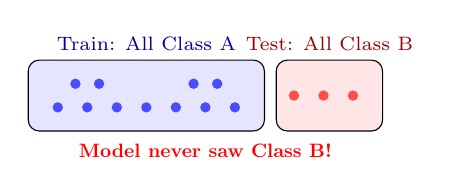
\begin{tikzpicture}[scale=0.75]
                % Train Box (Blue Region)
                \draw[fill=blue!10, rounded corners] (0,0) rectangle (4,1.2);
                \node[above, font=\scriptsize, blue!60!black] at (2,1.2) {Train: All Class A};
                \foreach \x in {0.5,1,1.5,2,2.5,3,3.5} \fill[blue!70] (\x, 0.4) circle (2.5pt);
                \foreach \x in {0.8,1.2,2.8,3.2} \fill[blue!70] (\x, 0.8) circle (2.5pt);
                
                % Test Box (Red Region)
                \draw[fill=red!10, rounded corners] (4.2,0) rectangle (6,1.2);
                \node[above, font=\scriptsize, red!60!black] at (5.1,1.2) {Test: All Class B};
                \foreach \x in {4.5,5,5.5} \fill[red!70] (\x, 0.6) circle (2.5pt);
                
                % Warning
                \node[below, red, font=\bfseries, scale=0.7] at (3, -0.1) {Model never saw Class B!};
            \end{tikzpicture}
            
            \vspace{1em}
            
            
        \end{column}
    \end{columns}

    
    
\end{frame}


% --- SLIDE 1: The Problem (Ordered Data) ---
\begin{frame}{The Problem: Ordered Data}
    
    \begin{columns}[c]
        % --- Left Column: The Logic ---
        \begin{column}{0.45\textwidth}
            \textbf{Data is Often Ordered}
            \begin{itemize}
                \item Real-world data is often collected sequentially (by date, time, or class).
                \item If we split data directly, the model trains on one pattern but gets tested on a completely different one.
            \end{itemize}
            
            \vspace{1em}
            \begin{block}{Solution: }Shuffle the data before splitting!
            \end{block}
        \end{column}
        
        % --- Right Column: The Visuals ---
        \begin{column}{0.55\textwidth}
            \centering
            
            \textbf{1. Ordered Split (Biased)}
            \vspace{0.2em}
            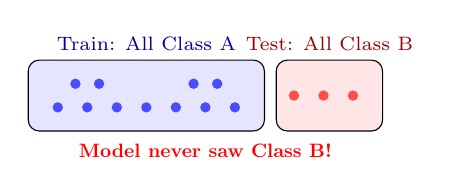
\begin{tikzpicture}[scale=0.75]
                % Train Box (Blue Region)
                \draw[fill=blue!10, rounded corners] (0,0) rectangle (4,1.2);
                \node[above, font=\scriptsize, blue!60!black] at (2,1.2) {Train: All Class A};
                \foreach \x in {0.5,1,1.5,2,2.5,3,3.5} \fill[blue!70] (\x, 0.4) circle (2.5pt);
                \foreach \x in {0.8,1.2,2.8,3.2} \fill[blue!70] (\x, 0.8) circle (2.5pt);
                
                % Test Box (Red Region)
                \draw[fill=red!10, rounded corners] (4.2,0) rectangle (6,1.2);
                \node[above, font=\scriptsize, red!60!black] at (5.1,1.2) {Test: All Class B};
                \foreach \x in {4.5,5,5.5} \fill[red!70] (\x, 0.6) circle (2.5pt);
                
                % Warning
                \node[below, red, font=\bfseries, scale=0.7] at (3, -0.1) {Model never saw Class B!};
            \end{tikzpicture}
            
            \vspace{1em}
            
            \textbf{2. Shuffled Split (Correct)}
            \vspace{0.2em}
            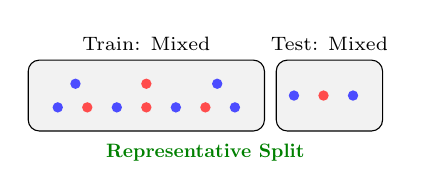
\begin{tikzpicture}[scale=0.75]
                % Train Box (Mixed)
                \draw[fill=gray!10, rounded corners] (0,0) rectangle (4,1.2);
                \node[above, font=\scriptsize] at (2,1.2) {Train: Mixed};
                % Mix of Blue and Red
                \foreach \x in {0.5,1.5,2.5,3.5} \fill[blue!70] (\x, 0.4) circle (2.5pt);
                \foreach \x in {1.0,2.0,3.0} \fill[red!70] (\x, 0.4) circle (2.5pt);
                \foreach \x in {0.8,3.2} \fill[blue!70] (\x, 0.8) circle (2.5pt);
                \foreach \x in {2.0} \fill[red!70] (\x, 0.8) circle (2.5pt);
                
                % Test Box (Mixed)
                \draw[fill=gray!10, rounded corners] (4.2,0) rectangle (6,1.2);
                \node[above, font=\scriptsize] at (5.1,1.2) {Test: Mixed};
                \fill[blue!70] (4.5, 0.6) circle (2.5pt);
                \fill[red!70] (5.0, 0.6) circle (2.5pt);
                \fill[blue!70] (5.5, 0.6) circle (2.5pt);
                
                % Success
                \node[below, green!50!black, font=\bfseries, scale=0.7] at (3, -0.1) { Representative Split \checkmark};
            \end{tikzpicture}
        \end{column}
    \end{columns}

    
    
\end{frame}

% --- SLIDE 1: The Problem (Ordered Data) ---
\begin{frame}{The Problem: Ordered Data}
    
    \begin{columns}[c]
        % --- Left Column: The Logic ---
        \begin{column}{0.45\textwidth}
            \textbf{Data is Often Ordered}
            \begin{itemize}
                \item Real-world data is often collected sequentially (by date, time, or class).
                \item If we split data directly, the model trains on one pattern but gets tested on a completely different one.
            \end{itemize}
            
            \vspace{1em}
            \begin{block}{Solution: }Shuffle the data before splitting!
            \end{block}
            \vspace{1em}
            \begin{block}{This helps, but what if data is small?}
            \end{block}
        \end{column}
        
        % --- Right Column: The Visuals ---
        \begin{column}{0.55\textwidth}
            \centering
            
            \textbf{1. Ordered Split (Biased)}
            \vspace{0.2em}
            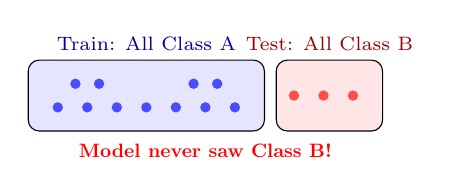
\begin{tikzpicture}[scale=0.75]
                % Train Box (Blue Region)
                \draw[fill=blue!10, rounded corners] (0,0) rectangle (4,1.2);
                \node[above, font=\scriptsize, blue!60!black] at (2,1.2) {Train: All Class A};
                \foreach \x in {0.5,1,1.5,2,2.5,3,3.5} \fill[blue!70] (\x, 0.4) circle (2.5pt);
                \foreach \x in {0.8,1.2,2.8,3.2} \fill[blue!70] (\x, 0.8) circle (2.5pt);
                
                % Test Box (Red Region)
                \draw[fill=red!10, rounded corners] (4.2,0) rectangle (6,1.2);
                \node[above, font=\scriptsize, red!60!black] at (5.1,1.2) {Test: All Class B};
                \foreach \x in {4.5,5,5.5} \fill[red!70] (\x, 0.6) circle (2.5pt);
                
                % Warning
                \node[below, red, font=\bfseries, scale=0.7] at (3, -0.1) {Model never saw Class B!};
            \end{tikzpicture}
            
            \vspace{1em}
            
            \textbf{2. Shuffled Split (Correct)}
            \vspace{0.2em}
            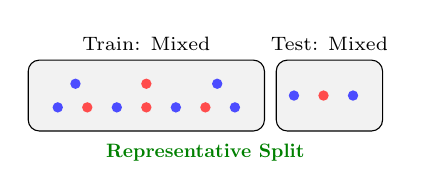
\begin{tikzpicture}[scale=0.75]
                % Train Box (Mixed)
                \draw[fill=gray!10, rounded corners] (0,0) rectangle (4,1.2);
                \node[above, font=\scriptsize] at (2,1.2) {Train: Mixed};
                % Mix of Blue and Red
                \foreach \x in {0.5,1.5,2.5,3.5} \fill[blue!70] (\x, 0.4) circle (2.5pt);
                \foreach \x in {1.0,2.0,3.0} \fill[red!70] (\x, 0.4) circle (2.5pt);
                \foreach \x in {0.8,3.2} \fill[blue!70] (\x, 0.8) circle (2.5pt);
                \foreach \x in {2.0} \fill[red!70] (\x, 0.8) circle (2.5pt);
                
                % Test Box (Mixed)
                \draw[fill=gray!10, rounded corners] (4.2,0) rectangle (6,1.2);
                \node[above, font=\scriptsize] at (5.1,1.2) {Test: Mixed};
                \fill[blue!70] (4.5, 0.6) circle (2.5pt);
                \fill[red!70] (5.0, 0.6) circle (2.5pt);
                \fill[blue!70] (5.5, 0.6) circle (2.5pt);
                
                % Success
                \node[below, green!50!black, font=\bfseries, scale=0.7] at (3, -0.1) { Representative Split \checkmark};
            \end{tikzpicture}
        \end{column}
    \end{columns}

    
    
\end{frame}

% --- SLIDE 2: But What If Data is Small? ---
\begin{frame}{What If Data is Small?}

    \begin{block}{The Remaining Problem}
        Shuffling fixes the \textit{order} bias, but with small datasets, a single random split can still be \textbf{unlucky}.
    \end{block}

    % \vspace{0.5em}
    
    \begin{columns}[c]
        % --- Left Column: Text Explanation (Narrower) ---
        \begin{column}{0.40\textwidth}
            \textbf{The Law of Small Numbers:}
            
            \begin{itemize}
                \item 20\% of a small dataset is a tiny sample.
                \item It is statistically likely that this small sample will not match the population perfectly.
                \item \textbf{Result:} We get "Lucky" or "Unlucky" splits.
            \end{itemize}
        \end{column}
        
        % --- Right Column: The Visuals (Wider) ---
        \begin{column}{0.65\textwidth}
            \centering
            
            % LEGEND (Centered)
            
\begin{tikzpicture}[scale=0.7]
                 \fill[blue!70] (0,0) circle (3pt); 
                 \node[right, scale=0.8] at (0.1,0) {Standard};
                 
                 \node[red, font=\bfseries] at (2.5,0) {x}; 
                 \node[right, scale=0.8] at (2.7,0) {Hard Case};
            \end{tikzpicture}
            
            \vspace{0.5em}
            
            % SCENARIO A: LUCKY
            \textbf{Scenario A: "Lucky" Split}
            \vspace{0.2em}
            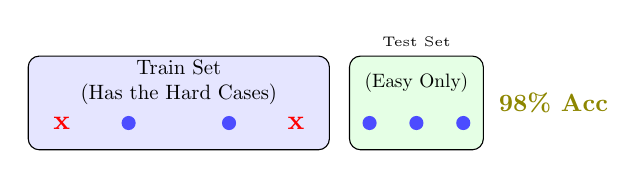
\begin{tikzpicture}[scale=0.85]
                % Train Box (Stretched width to 4.5)
                \draw[fill=blue!10, rounded corners] (0,0) rectangle (4.5,1.4);
                % Text Centered
                \node[scale=0.75, align=center] at (2.25, 1.0) {Train Set\\(Has the Hard Cases)};
                % Markers spread out
                \node[red, font=\bfseries] at (0.5,0.4) {x}; 
                \node[red, font=\bfseries] at (4.0,0.4) {x};
                \fill[blue!70] (1.5,0.4) circle (3pt);
                \fill[blue!70] (3.0,0.4) circle (3pt);
                
                % Test Box (Stretched & Shifted)
                \draw[fill=green!10, rounded corners] (4.8,0) rectangle (6.8,1.4);
                \node[above, font=\tiny] at (5.8,1.4) {Test Set};
                \node[scale=0.7, align=center] at (5.8, 1.0) {(Easy Only)};
                % Test has ONLY Blue Dots
                \fill[blue!70] (5.1, 0.4) circle (3pt); 
                \fill[blue!70] (5.8, 0.4) circle (3pt); 
                \fill[blue!70] (6.5, 0.4) circle (3pt);
                
                \node[right, olive, font=\bfseries, scale=0.9] at (6.9, 0.7) {98\% Acc};
            \end{tikzpicture}
            
            \vspace{0.8em}
            
            % SCENARIO B: UNLUCKY
            \textbf{Scenario B: "Unlucky" Split}
            \vspace{0.2em}
            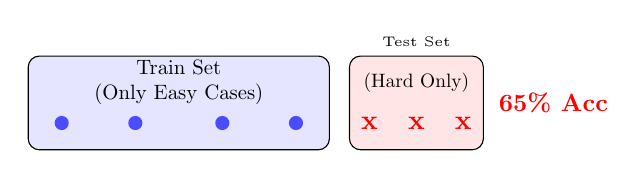
\begin{tikzpicture}[scale=0.85]
                % Train Box
                \draw[fill=blue!10, rounded corners] (0,0) rectangle (4.5,1.4);
                % Text Centered
                \node[scale=0.75, align=center] at (2.25, 1.0) {Train Set\\(Only Easy Cases)};
                % Markers spread out
                \fill[blue!70] (0.5,0.4) circle (3pt); 
                \fill[blue!70] (1.6,0.4) circle (3pt); 
                \fill[blue!70] (2.9,0.4) circle (3pt);
                \fill[blue!70] (4.0,0.4) circle (3pt);
                
                % Test Box
                \draw[fill=red!10, rounded corners] (4.8,0) rectangle (6.8,1.4);
                \node[above, font=\tiny] at (5.8,1.4) {Test Set};
                \node[scale=0.7, align=center] at (5.8, 1.0) {(Hard Only)};
                % Test has THE RED Xs
                \node[red, font=\bfseries] at (5.1, 0.4) {x}; 
                \node[red, font=\bfseries] at (5.8, 0.4) {x}; 
                \node[red, font=\bfseries] at (6.5, 0.4) {x};
                
                \node[right, red, font=\bfseries, scale=0.9] at (6.9, 0.7) {65\% Acc};
            \end{tikzpicture}
            
            \vspace{0.5em}
            {\small\textit{Same data, just a different random cut!}}
        \end{column}
    \end{columns}
\end{frame}

\definecolor{darkred}{rgb}{0.5,0,0}
\definecolor{darkblue}{RGB}{0,0,139}


% --- SLIDE 3: K-FOLD SOLUTION ---
\begin{frame}{The Solution: K-Fold Cross Validation}

    \textbf{Use ALL Data for Testing (Across Multiple Rounds)}
    \begin{enumerate}
        \item Split shuffled data into $K$ equal folds (e.g., $K=5$).
        \item Train on $K-1$, test on the remaining 1.
        \item \textbf{Rotate} until every fold has been the test set exactly once.
        \item \textbf{Average} the scores.
    \end{enumerate}

    \vspace{0.5em}
    \centering
    
    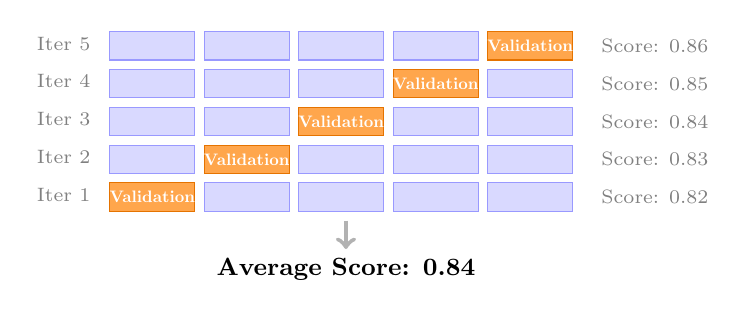
\begin{tikzpicture}[scale=0.6]
        \foreach \y in {0,1,2,3,4} {
             \node[left, font=\scriptsize, gray] at (-0.2, \y*0.8 + 0.35) {Iter \the\numexpr\y+1};
             \foreach \x in {0,1,2,3,4} {
                \ifnum \x=\y
                    % Test Fold
                    \draw[fill=orange!70, draw=orange!90!black] (\x*2, \y*0.8) rectangle (\x*2+1.8, \y*0.8+0.6);
                    \node[scale=0.6, font=\bfseries, white] at (\x*2+0.9, \y*0.8+0.3) {Validation};
                \else
                    % Train Fold
                    \draw[fill=blue!15, draw=blue!40] (\x*2, \y*0.8) rectangle (\x*2+1.8, \y*0.8+0.6);
                \fi
             }
             \node[right, font=\scriptsize, gray] at (10.2, \y*0.8+0.3) {Score: 0.\the\numexpr82+\y};
        }
        
        % Average Visual
        \draw[->, ultra thick, gray!60] (5, -0.2) -- (5, -0.8);
        \node[below, black, align=center, font=\small\bfseries] at (5, -0.8) {Average Score: 0.84};
    \end{tikzpicture}
\end{frame}

% --- SLIDE 3: K-FOLD SOLUTION ---
\begin{frame}{The Solution: K-Fold Cross Validation}

    \begin{tcolorbox}[colback=darkblue!5, colframe=darkblue!90, title=Why K-Fold Works]
        Every data point serves as a test sample exactly once. We evaluate on \textbf{100\%} of the data instead of just 20\%, removing the luck factor.
    \end{tcolorbox}

    \vspace{1.5em}
    \centering
    
    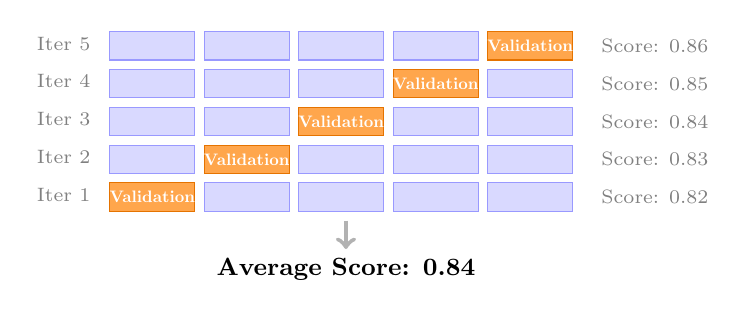
\begin{tikzpicture}[scale=0.6]
        \foreach \y in {0,1,2,3,4} {
             \node[left, font=\scriptsize, gray] at (-0.2, \y*0.8 + 0.35) {Iter \the\numexpr\y+1};
             \foreach \x in {0,1,2,3,4} {
                \ifnum \x=\y
                    % Test Fold
                    \draw[fill=orange!70, draw=orange!90!black] (\x*2, \y*0.8) rectangle (\x*2+1.8, \y*0.8+0.6);
                    \node[scale=0.6, font=\bfseries, white] at (\x*2+0.9, \y*0.8+0.3) {Validation};
                \else
                    % Train Fold
                    \draw[fill=blue!15, draw=blue!40] (\x*2, \y*0.8) rectangle (\x*2+1.8, \y*0.8+0.6);
                \fi
             }
             \node[right, font=\scriptsize, gray] at (10.2, \y*0.8+0.3) {Score: 0.\the\numexpr82+\y};
        }
        
        % Average Visual
        \draw[->, ultra thick, gray!60] (5, -0.2) -- (5, -0.8);
        \node[below, black, align=center, font=\small\bfseries] at (5, -0.8) {Average Score: 0.84};
    \end{tikzpicture}
    
\end{frame}

% --- SLIDE 3: K-FOLD SOLUTION ---
\begin{frame}{The Solution: K-Fold Cross Validation}

    \begin{tcolorbox}[colback=darkblue!5, colframe=darkblue!90, title=Why K-Fold Works]
        Every data point serves as a test sample exactly once. We evaluate on \textbf{100\%} of the data instead of just 20\%, removing the luck factor.
    \end{tcolorbox}

    \vspace{1.5em}
    \centering
    
    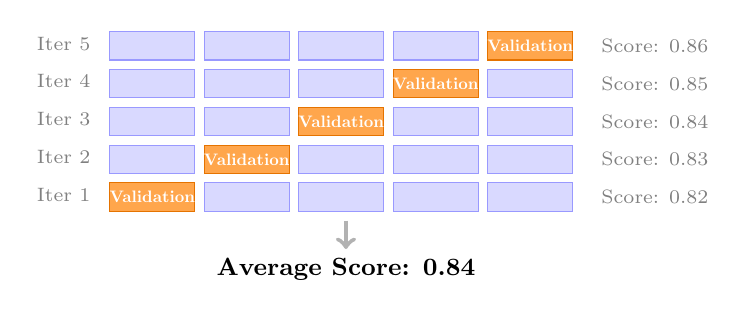
\begin{tikzpicture}[scale=0.6]
        \foreach \y in {0,1,2,3,4} {
             \node[left, font=\scriptsize, gray] at (-0.2, \y*0.8 + 0.35) {Iter \the\numexpr\y+1};
             \foreach \x in {0,1,2,3,4} {
                \ifnum \x=\y
                    % Test Fold
                    \draw[fill=orange!70, draw=orange!90!black] (\x*2, \y*0.8) rectangle (\x*2+1.8, \y*0.8+0.6);
                    \node[scale=0.6, font=\bfseries, white] at (\x*2+0.9, \y*0.8+0.3) {Validation};
                \else
                    % Train Fold
                    \draw[fill=blue!15, draw=blue!40] (\x*2, \y*0.8) rectangle (\x*2+1.8, \y*0.8+0.6);
                \fi
             }
             \node[right, font=\scriptsize, gray] at (10.2, \y*0.8+0.3) {Score: 0.\the\numexpr82+\y};
        }
        
        % Average Visual
        \draw[->, ultra thick, gray!60] (5, -0.2) -- (5, -0.8);
        \node[below, black, align=center, font=\small\bfseries] at (5, -0.8) {Average Score: 0.84};
    \end{tikzpicture}

    \begin{itemize}
                \item Only one problem left...
            \end{itemize}

    
    
\end{frame}



% --- SLIDE 1: IMBALANCE MOTIVATION (The Accuracy Paradox) ---
\begin{frame}{The Hidden Trap: Imbalanced Data}

    \begin{columns}[c]
        % --- Left Column: The Concept ---
        \begin{column}{0.45\textwidth}
            \textbf{What is Imbalance?}
            \begin{itemize}
                \item When one class dominates the target (e.g., 99\% Healthy, 1\% Sick).
            \end{itemize}
            
            \vspace{1em}
            \begin{alertblock}{The Accuracy Paradox}
                If you have 99 blue dots and 1 red dot, a model that \textbf{always guesses Blue} has 99\% Accuracy!
                \vspace{0.5em}
                
                But it failed to find the one thing we cared about!
            \end{alertblock}
        \end{column}
        
        % --- Right Column: The Visual ---
        \begin{column}{0.55\textwidth}
            \centering
            
            % 1. The Full Dataset
            \textbf{1. Target Distribution} \\(95\% Blue, 5\% Red)
            \vspace{0.2em}
            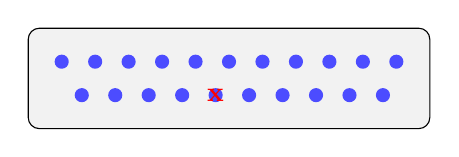
\begin{tikzpicture}[scale=0.85]
                \draw[fill=gray!10, rounded corners] (0,0) rectangle (6,1.5);
                % Lots of Blue
                \foreach \x in {0.5,1.0,1.5,2.0,2.5,3.0,3.5,4.0,4.5,5.0,5.5} 
                    \fill[blue!70] (\x, 1.0) circle (3pt);
                \foreach \x in {0.8,1.3,1.8,2.3,2.8,3.3,3.8,4.3,4.8,5.3} 
                    \fill[blue!70] (\x, 0.5) circle (3pt);
                
                % One tiny Red dot (The Needle)
                \node[red, font=\bfseries] at (2.8, 0.5) {x};
            \end{tikzpicture}
            
            \vspace{0.8em}
            
            % 2. Random Split Failure
            \textbf{2. Random Split}
            \vspace{0.2em}
            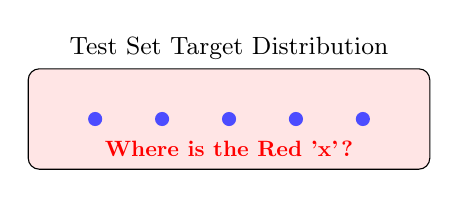
\begin{tikzpicture}[scale=0.85]
                % Test Set Box
                \draw[fill=red!10, rounded corners] (0,0) rectangle (6,1.5);
                \node[above, font=\small] at (3,1.5) {Test Set Target Distribution};
                
                % It picked only Blue
                \foreach \x in {1.0, 2.0, 3.0, 4.0, 5.0} 
                    \fill[blue!70] (\x, 0.75) circle (3pt);
                
                % Warning Label
                \node[red, font=\bfseries, scale=0.8] at (3, 0.3) {Where is the Red 'x'?};
            \end{tikzpicture}
  
        \end{column}
    \end{columns}
\end{frame}

% --- SLIDE 2: STRATIFICATION (The Solution) ---
\begin{frame}{The Fix: Stratified Splitting}

    \begin{block}{Definition}
        \textbf{Stratification} forces the Train and Test splits to preserve the \textbf{same class ratios} as the original dataset.
    \end{block}

    \vspace{1em}
    \centering
    
    \begin{columns}[c]
        % Visualizing the Force Split
        \begin{column}{0.6\textwidth}
            \centering
            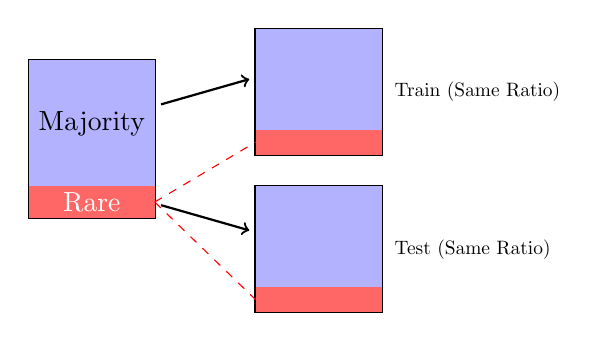
\begin{tikzpicture}[scale=0.8]
                % Full Data
                \draw[thick] (0,0) rectangle (2,2.5);
                \fill[blue!30] (0,0.5) rectangle (2,2.5); \node at (1,1.5) {Majority};
                \fill[red!60] (0,0) rectangle (2,0.5); \node[white] at (1,0.25) {Rare};
                
                % Arrows
                \draw[->, thick] (2.1, 1.8) -- (3.5, 2.2);
                \draw[->, thick] (2.1, 0.2) -- (3.5, -0.2);
                
                % Train
                \draw[thick, fill=blue!10] (3.6, 1.0) rectangle (5.6, 3.0);
                \fill[blue!30] (3.6, 1.4) rectangle (5.6, 3.0);
                \fill[red!60] (3.6, 1.0) rectangle (5.6, 1.4);
                \node[right, scale=0.7] at (5.7, 2.0) {Train (Same Ratio)};
                
                % Test
                \draw[thick, fill=blue!10] (3.6, -1.5) rectangle (5.6, 0.5);
                \fill[blue!30] (3.6, -1.1) rectangle (5.6, 0.5);
                \fill[red!60] (3.6, -1.5) rectangle (5.6, -1.1);
                \node[right, scale=0.7] at (5.7, -0.5) {Test (Same Ratio)};
                
                % Connection Lines indicating forced movement
                \draw[dashed, red] (2, 0.25) -- (3.6, 1.2);
                \draw[dashed, red] (2, 0.25) -- (3.6, -1.3);
            \end{tikzpicture}
        \end{column}
        
        % Text Explanation
        \begin{column}{0.4\textwidth}
            \textbf{Why it works:}
            \begin{itemize}
                \item It guarantees the Test set includes the "Red 'x'".
                \item It allows us to calculate metrics like Recall and F1-Score properly.
            \end{itemize}
            
            \vspace{1em}
            \begin{tcolorbox}[colback=green!5, colframe=green!40]
                \centering \small
                \textbf{Tip:}\\
                Use \textbf{Stratified K-Fold} for the best of both worlds!
            \end{tcolorbox}
        \end{column}
    \end{columns}
    
\end{frame}


\subsection{Performance Measurements (Metrics)}

\begin{frame}{Addressing Overfitting}
    \centering
    \large \textit{Since we cannot trust the training error, we need a systematic approach to validate our models.}
    
    \vspace{0.8cm}
    
    \begin{columns}[T]
        \begin{column}{0.3\textwidth}
            \begin{block}{\centering1. Detect:}
                \centering
                \textbf{Splitting Data}\\
                (Holdout, K-Fold)
            \end{block}
        \end{column}
        \begin{column}{0.3\textwidth}
            \begin{block}{\centering2. Measure:}
                \centering
                \textbf{Metrics}\\
                (Accuracy, MSE, F1, AUC)
            \end{block}
        \end{column}
        \begin{column}{0.3\textwidth}
            \begin{block}{\centering3. Mitigate:}
                \centering
                \textbf{Strategies}\\
                (Regularization, More Data, Better Features)
            \end{block}
        \end{column}
    \end{columns}
    
    \vspace{0.5cm}
    \centering
    \small $\rightarrow$ \textit{Step 1: How to simulate "unseen data" using Splits.} \\
    \small $\rightarrow$ \textit{Step 2: How to measure performance using Metrics.}
\end{frame}

% --- PART 2: MEASUREMENT ---


% --- SLIDE 1: INTRO (What & Why) ---
\begin{frame}{Measuring Performance: Metrics}

    \begin{block}{Definition}
        A \textbf{Metric} is a quantifiable measure used to evaluate how well a model is performing on a specific task.
    \end{block}

    % \vspace{-2em}
    
    \textbf{Loss Function vs. Metric}
    \vspace{-1em}
    
    \begin{columns}[T]
        \begin{column}{0.49\textwidth}
            \begin{tcolorbox}[colback=blue!5, colframe=blue!50, title=Loss (For the Machine)]
                \small
                \begin{itemize}
                    \item Used during \textbf{Training}.
                    \item Must be \textbf{Differentiable} (smooth) so we can calculate gradients.
                    \item \textit{Example: Cross-Entropy, MSE.}
                \end{itemize}
            \end{tcolorbox}
        \end{column}
        
        \begin{column}{0.49\textwidth}
            \begin{tcolorbox}[colback=darkred!5, colframe=darkred!90, title=Metric (For the Human)]
                \small
                \begin{itemize}
                    \item Used during \textbf{Evaluation} (Validation/Test).
                    \item Must be \textbf{Interpretable} by humans (business value).
                    \item \textit{Example: Accuracy, F1-Score, Dollar Amount.}
                \end{itemize}
            \end{tcolorbox}
        \end{column}
    \end{columns}
\end{frame}

\begin{frame}{Measuring Performance: Metrics}

    \begin{block}{Definition}
        A \textbf{Metric} is a quantifiable measure used to evaluate how well a model is performing on a specific task.
    \end{block}

    % \vspace{-2em}
    
    \textbf{Loss Function vs. Metric}
    \vspace{-1em}
    
    \begin{columns}[T]
        \begin{column}{0.49\textwidth}
            \begin{tcolorbox}[colback=blue!5, colframe=blue!50, title=Loss (For the Machine)]
                \small
                \begin{itemize}
                    \item Used during \textbf{Training}.
                    \item Must be \textbf{Differentiable} (smooth) so we can calculate gradients.
                    \item \textit{Example: Cross-Entropy, MSE.}
                \end{itemize}
            \end{tcolorbox}
        \end{column}
        
        \begin{column}{0.49\textwidth}
            \begin{tcolorbox}[colback=darkred!5, colframe=darkred!90, title=Metric (For the Human)]
                \small
                \begin{itemize}
                    \item Used during \textbf{Evaluation} (Validation/Test).
                    \item Must be \textbf{Interpretable} by humans (business value).
                    \item \textit{Example: Accuracy, F1-Score, Dollar Amount.}
                \end{itemize}
            \end{tcolorbox}
        \end{column}
    \end{columns}
    
    % \vspace{1em}
    \centering
    \textit{Metrics differ based on the task: Regression (Numbers) vs. Classification (Classes).}
\end{frame}


% --- SLIDE 2: REGRESSION METRICS ---
% --- SLIDE 1: FORMULAS & INTUITION ---
\begin{frame}{Metrics for Regression: MAE vs. MSE}

    \begin{columns}[T]
        % --- MAE Column ---
        \begin{column}{0.48\textwidth}
            \begin{block}{Mean Absolute Error (MAE)}
                \centering
                $$ \text{MAE} = \frac{1}{n} \sum |y - \hat{y}| $$
                \begin{itemize}
                    \item Measures average absolute distance.
                    \item \textbf{Robust:} Treats all errors linearly.
                \end{itemize}
            \end{block}
        \end{column}
        
        % --- MSE Column ---
        \begin{column}{0.48\textwidth}
            \begin{block}{Mean Squared Error (MSE)}
                \centering
                $$ \text{MSE} = \frac{1}{n} \sum (y - \hat{y})^2 $$
                \begin{itemize}
                    \item Squares the difference.
                    \item \textbf{Sensitive to outliers:} Large errors are punished heavily ($10^2 = 100$).
                    \item Easy to differentiate.
                \end{itemize}
            \end{block}
        \end{column}
    \end{columns}

\end{frame}

% --- SLIDE 2: INTERPRETATION EXAMPLE ---
\begin{frame}{Interpreting the Score}

    \textbf{Scenario:} You are training a model to predict \textbf{House Prices}.
    
    \vspace{1em}
    
    \begin{columns}[T]
        % --- MAE Interpretation ---
        \begin{column}{0.48\textwidth}
            \begin{tcolorbox}[colback=blue!5, colframe=blue!50, title={$MAE = 10{,}000$}]
                \textbf{What it means:}
                \vspace{0.5em}
                \begin{itemize}
                    \item "On average, my prediction is off by \textbf{\$10,000}."
                \end{itemize}
                \vspace{0.5em}
                \textit{Easy to explain.}
            \end{tcolorbox}
        \end{column}
        
        % --- MSE Interpretation ---
        \begin{column}{0.48\textwidth}
            \begin{tcolorbox}[colback=darkred!5, colframe=darkred!90, title={$MSE = 100{,}000{,}000$}]
                \textbf{What it means:}
                \vspace{0.5em}
                \begin{itemize}
                    \item The unit is \textbf{"Dollars Squared"} ($\$^{2}$).
                    \item Hard to interpret directly!
                    \item \textbf{Why use it?} To force the model to focus on fixing the massive mistakes first.
                \end{itemize}
            \end{tcolorbox}
        \end{column}
    \end{columns}
    
    \centering
    \small \textbf{Common Fix:} Take the square root ($\sqrt{MSE}$) to get \textbf{RMSE}, which brings the units back to dollars.
\end{frame}

% --- SLIDE 1: ACCURACY DEFINITION ---
\begin{frame}{Metrics for Classification: Accuracy}
    \centering
    \begin{block}{Definition}
        The percentage of predictions that our model got correct.
    \end{block}
        
    \[
        \text{Accuracy} = \frac{\text{Number of Correct Predictions}}{\text{Total Number of Predictions}}
    \]
\end{frame}

\begin{frame}{Metrics for Classification: Accuracy}
    \centering
    \begin{block}{Definition}
        The percentage of predictions that our model got correct.
    \end{block}
        
    \[
        \text{Accuracy} = \frac{\text{Number of Correct Predictions}}{\text{Total Number of Predictions}}
    \]

    \small \textit{Q: Can we use it as a loss?}
\end{frame}

\begin{frame}{Metrics for Classification: Accuracy}
    \centering
    \begin{block}{Definition}
        The percentage of predictions that our model got correct.
    \end{block}
        
    \[
        \text{Accuracy} = \frac{\text{Number of Correct Predictions}}{\text{Total Number of Predictions}}
    \]

    \small \textit{Q: Can we use it as a loss? }\textbf{No, non-differentiable.}
\end{frame}

\begin{frame}{Metrics for Classification: Accuracy}
    \centering
    \begin{block}{Definition}
        The percentage of predictions that our model got correct.
    \end{block}
        
    \[
        \text{Accuracy} = \frac{\text{Number of Correct Predictions}}{\text{Total Number of Predictions}}
    \]

    \small \textit{Accuracy works well until you work with an imbalance target. Can you figure out why?}
\end{frame}


% --- SLIDE 3: THE IMBALANCE TRAP ---
\begin{frame}{When Accuracy Fails: Imbalanced Data}

        Imagine a dataset where \textbf{99\%} of samples are Class A and only \textbf{1\%} are Class B.

    \vspace{1.5em}

    \begin{columns}[c]
        \begin{column}{0.6\textwidth}
            \textbf{Scenario:}
            \begin{itemize}
                \item We build a "Lazy Model" that ignores the data and always predicts \textbf{"Class A"}.
            \end{itemize}
        \end{column}
        
        \begin{column}{0.4\textwidth}
            \centering
            \begin{tcolorbox}[colback=red!5, colframe=red!60, boxrule=0.5pt]
                \centering \textbf{Result:}\\
                \Huge 99\% \\ 
                \normalsize Accuracy
            \end{tcolorbox}
        \end{column}
    \end{columns}

    \vspace{1.5em}
    \centering
    \begin{block}{The model is useless (it never finds Class B), but Accuracy says it's amazing. We need better metrics to evaluate its performance against the minority class.}
    \end{block}
\end{frame}

% --- SLIDE 4: CONFUSION MATRIX (CLEANER) ---
\begin{frame}{The Foundation: Confusion Matrix}
    \centering
    \textit{To understand the errors, we break them down into a table.}
    
    \vspace{0.5em}

    % A cleaner, more spaced out matrix
    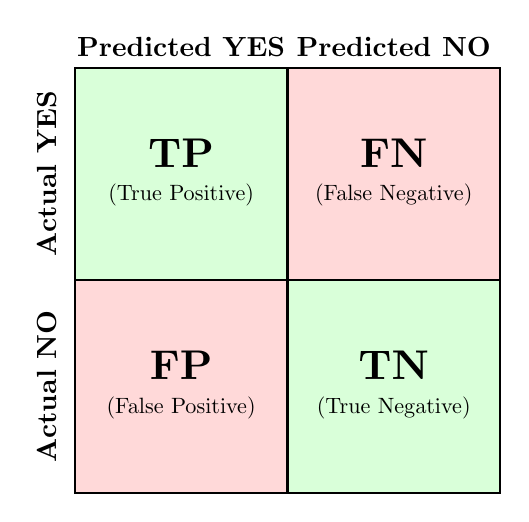
\begin{tikzpicture}[scale=0.9]
        % Labels
        \node[font=\bfseries] at (1.5, 3.3) {Predicted YES};
        \node[font=\bfseries] at (4.5, 3.3) {Predicted NO};
        \node[rotate=90, font=\bfseries] at (-0.4, 1.5) {Actual YES};
        \node[rotate=90, font=\bfseries] at (-0.4, -1.5) {Actual NO};

        % Boxes
        % TP (Green)
        \draw[fill=green!15, thick] (0,0) rectangle (3,3);
        \node[scale=1.5, font=\bfseries] at (1.5, 1.8) {TP};
        \node[scale=0.8] at (1.5, 1.2) {(True Positive)};
        
        % FN (Red)
        \draw[fill=red!15, thick] (3,0) rectangle (6,3);
        \node[scale=1.5, font=\bfseries] at (4.5, 1.8) {FN};
        \node[scale=0.8] at (4.5, 1.2) {(False Negative)};
        
        % FP (Orange)
        \draw[fill=red!15, thick] (0,-3) rectangle (3,0);
        \node[scale=1.5, font=\bfseries] at (1.5, -1.2) {FP};
        \node[scale=0.8] at (1.5, -1.8) {(False Positive)};
        
        % TN (Green)
        \draw[fill=green!15, thick] (3,-3) rectangle (6,0);
        \node[scale=1.5, font=\bfseries] at (4.5, -1.2) {TN};
        \node[scale=0.8] at (4.5, -1.8) {(True Negative)};
    \end{tikzpicture}
\end{frame}

% --- SLIDE 5: PRECISION ---
\begin{frame}{Metric: Precision}
    
    \begin{block}{Question}
        \textit{"Of all the times the model predicted \textbf{YES}, how often was it right?"}
    \end{block}

    \vspace{1em}
    
    \[
        \text{Precision} = \frac{\text{True Positives}}{\text{True Positives} + \textbf{False Positives}}
    \]
    
    \vspace{1.5em}
    
    \textbf{When to use it?}
    \begin{itemize}
        \item When \textbf{False Positives} are expensive/annoying.
        \item \textbf{Example: Spam Filter.} 
        \item We do \textbf{not} want to mark a real email (work, family) as Spam. Better to let a few spam emails through than delete a real one.
    \end{itemize}

\end{frame}

% --- SLIDE 6: RECALL ---
\begin{frame}{Metric: Recall}
    
    \begin{block}{Question}
        \textit{"Of all the \textbf{Real YES} cases in the world, how many did we find?"}
    \end{block}

    \vspace{1em}
    
    \[
        \text{Recall} = \frac{\text{True Positives}}{\text{True Positives} + \textbf{False Negatives}}
    \]
    
    \vspace{1.5em}
    
    \textbf{When to use it?}
    \begin{itemize}
        \item When \textbf{False Negatives} are dangerous/fatal.
        \item \textbf{Example: Cancer/Fraud Detection.} 
        \item We must find \textbf{every} sick patient. It is okay to raise a false alarm (do more tests), but we cannot miss a sick person.
    \end{itemize}

\end{frame}

% --- SLIDE 7: F1 SCORE ---
\begin{frame}{Metric: F1-Score}

    \begin{itemize}
        \item Often we need a balance between Precision and Recall.
        \item If you optimize only one, the other usually suffers (Precision-Recall Tradeoff).
    \end{itemize}

    \vspace{1em}
    
    \begin{block}{F1-Score (Harmonic Mean of Precision and Recall)}
        \[
            F1 = 2 \times \frac{\text{Precision} \times \text{Recall}}{\text{Precision} + \text{Recall}}
        \]
    \end{block}
    
    \begin{itemize}
        \item Used for imbalanced data.
    \end{itemize}
    
    \textbf{Why Harmonic Mean not Arithmetic Mean?}
    \begin{itemize}
        \item It forces the model to be good at \textbf{both}. If Precision is 100\% but Recall is 0\%, the Average is 50\%, but the \textbf{F1-Score is 0}.
    \end{itemize}

\end{frame}

% --- SLIDE 6: BASELINE ---

\begin{frame}{How to know if a specific score is good?}

    \textbf{Question:} My F1-Score is 40\%. Is that good?
\end{frame}
    
\begin{frame}{Baselines}

    \textbf{Question:} My F1-Score is 40\%. Is that good?
    \vspace{0.5em}
    \\
    \textbf{Answer:} Compare it to a "Dummy" Baseline!
    
    \vspace{1em}
    
    \begin{columns}[T]
        \begin{column}{0.48\textwidth}
            \textbf{Classification Baseline}
            \begin{itemize}
                \item Always predict the \textbf{Majority Class}.
                \item If your model can't beat this, it hasn't learned anything.
            \end{itemize}
        \end{column}
        \begin{column}{0.48\textwidth}
            \textbf{Regression Baseline}
            \begin{itemize}
                \item MSE baseline: Use the \textbf{Mean}.
                \item MAE baseline: Use the \textbf{Median}.
                \item If your model can't beat this, you are doing worse than just guessing the average/median!
            \end{itemize}
        \end{column}
    \end{columns}
    
\end{frame}

\subsection{Overfitting Mitigation}

\begin{frame}{Addressing Overfitting}
    \centering
    \large \textit{Since we cannot trust the training error, we need a systematic approach to validate our models.}
    
    \vspace{0.8cm}
    
    \begin{columns}[T]
        \begin{column}{0.3\textwidth}
            \begin{block}{\centering1. Detect:}
                \centering
                \textbf{Splitting Data}\\
                (Holdout, K-Fold)
            \end{block}
        \end{column}
        \begin{column}{0.3\textwidth}
            \begin{block}{\centering2. Measure:}
                \centering
                \textbf{Metrics}\\
                (Accuracy, MSE, F1, AUC)
            \end{block}
        \end{column}
        \begin{column}{0.3\textwidth}
            \begin{block}{\centering3. Mitigate:}
                \centering
                \textbf{Strategies}\\
                (Regularization, More Data, Better Features)
            \end{block}
        \end{column}
    \end{columns}
    
    \vspace{0.5cm}
    \centering
    \small $\rightarrow$ \textit{Step 1: How to simulate "unseen data" using Splits.} \\
    \small $\rightarrow$ \textit{Step 2: How to measure performance using Metrics.} \\
    \small $\rightarrow$ \textit{Step 3: How to mitigate overfitting.}
\end{frame}

% --- PART 3: REDUCTION (Fixes) ---
% --- PART 3: REDUCTION (MITIGATION) ---
% --- PART 3: REDUCTION (MITIGATION) ---


% --- SLIDE 1: MODEL COMPLEXITY & HYPERPARAMETERS ---
\begin{frame}{Hyperparameters: Capacity \& Optimization}

    \begin{block}{}
        \textbf{Hyperparameters} are settings chosen \textbf{before} training.
        \begin{itemize}
            \item \textbf{Structural:} Control model complexity/capacity (e.g., Tree Depth, Layers).
            \item \textbf{Optimization:} Control the training process (e.g., Learning Rate).
        \end{itemize}
    \end{block}

    \vspace{0.5em}
    \centering
    
    % --- PART A: STRUCTURAL (Capacity) ---
    \textbf{A. Structural Params (Controlling Overfitting)}
    \begin{columns}[T]
        \begin{column}{0.48\textwidth}
            \begin{tcolorbox}[colback=blue!5, colframe=blue!50, title=Rigid (Risk: Underfitting), fonttitle=\small, left=2pt, right=2pt]
                \footnotesize
                \begin{itemize}
                    \item Poly Degree = 1 (Line)
                    \item Tree Depth = 1 (Stump)
                    \item NN Layers = 1 (Shallow)
                \end{itemize}
            \end{tcolorbox}
        \end{column}
        
        \begin{column}{0.48\textwidth}
            \begin{tcolorbox}[colback=red!5, colframe=red!50, title=Flexible (Risk: Overfitting), fonttitle=\small, left=2pt, right=2pt]
                \footnotesize
                \begin{itemize}
                    \item Poly Degree = 20 (Wiggly)
                    \item Tree Depth = 100 (Deep)
                    \item NN Layers = 20 (Deep)
                \end{itemize}
            \end{tcolorbox}
        \end{column}
    \end{columns}
  

\end{frame}

\begin{frame}{Hyperparameters: Capacity \& Optimization}

    \begin{block}{}
        \textbf{Hyperparameters} are settings chosen \textbf{before} training.
        \begin{itemize}
            \item \textbf{Structural:} Control model complexity/capacity (e.g., Tree Depth, Layers).
            \item \textbf{Optimization:} Control the training process (e.g., Learning Rate).
        \end{itemize}
    \end{block}

    \vspace{0.5em}
    \centering
    
    % --- PART B: OPTIMIZATION (Speed/Stability) ---
    \textbf{B. Optimization Params (The "Learning" Process)}
    \begin{tcolorbox}[colback=gray!10, colframe=gray!60, boxrule=0.5pt]
        \centering
        \small
        \textbf{Learning Rate (LR):} The "Step Size" of the update.
        \vspace{0.3em}
        \begin{columns}[c]
            \begin{column}{0.33\textwidth}
                \centering \scriptsize \textbf{Too Low} \\ $\to$ Slow/Stuck
            \end{column}
            \begin{column}{0.33\textwidth}
                \centering \scriptsize \textbf{Just Right} \\ $\to$ Converges
            \end{column}
            \begin{column}{0.33\textwidth}
                \centering \scriptsize \textbf{Too High} \\ $\to$ Unstable/Diverges
            \end{column}
        \end{columns}
    \end{tcolorbox}

\end{frame}



% --- SLIDE 2: MITIGATION STRATEGIES ---
% --- SLIDE 1: STRATEGY A (DATA) ---
\begin{frame}{Increase Data Size}
    \begin{block}{The Logic}
        Overfitting happens when the model memorizes "noise" in the gaps between data points. 
        \textbf{Solution:} Fill the gaps with more data.
    \end{block}
    \vspace{0.8em}
    \centering
    
    \begin{columns}[T]
        % --- Small Data ---
        \begin{column}{0.50\textwidth}
            \centering
            \textbf{1. Small Data (Sparse)}
            \vspace{0.5em}
            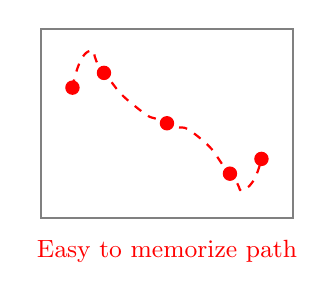
\begin{tikzpicture}[scale=0.8]
                % Box
                \draw[thick, gray] (0,0) rectangle (4,3);
                % 5 Points - positioned at extremes to look unrepresentative when sparse
                \filldraw[red] (0.5, {1.5 + 0.8*sin(0.5*90)}) circle (3pt);
                \filldraw[red] (1.0, {1.5 + 0.8*sin(1.0*90)}) circle (3pt);  % near peak
                \filldraw[red] (2.0, {1.5 + 0.8*sin(2.0*90)}) circle (3pt);
                \filldraw[red] (3.0, {1.5 + 0.8*sin(3.0*90)}) circle (3pt);  % near trough
                \filldraw[red] (3.5, {1.5 + 0.8*sin(3.5*90)}) circle (3pt);
                
                % Dashed line showing "Memorization" - overly wiggly overfitting
                \draw[red, dashed, thick] plot[smooth, tension=1.2] coordinates {
                    (0.5, {1.5 + 0.8*sin(0.5*90)}) 
                    (0.75, {1.5 + 0.8*sin(0.75*90) + 0.4})
                    (1.0, {1.5 + 0.8*sin(1.0*90)}) 
                    (1.5, {1.5 + 0.8*sin(1.5*90) - 0.3})
                    (2.0, {1.5 + 0.8*sin(2.0*90)}) 
                    (2.5, {1.5 + 0.8*sin(2.5*90) + 0.35})
                    (3.0, {1.5 + 0.8*sin(3.0*90)}) 
                    (3.25, {1.5 + 0.8*sin(3.25*90) - 0.3})
                    (3.5, {1.5 + 0.8*sin(3.5*90)})
                };
                
                \node[below, red, font=\small] at (2,-0.2) {Easy to memorize path};
            \end{tikzpicture}
        \end{column}
        
        % --- Large Data ---
        \begin{column}{0.50\textwidth}
            \centering
            \textbf{2. Large Data (Dense)}
            \vspace{0.5em}
            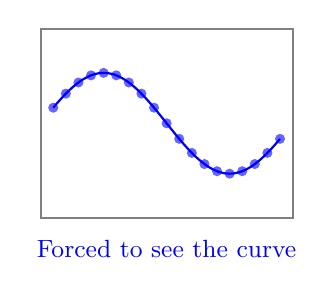
\begin{tikzpicture}[scale=0.8]
                % Box
                \draw[thick, gray] (0,0) rectangle (4,3);
                % Many points following a sine pattern
                \foreach \x in {0.2,0.4,0.6,0.8,1.0,1.2,1.4,1.6,1.8,2.0,2.2,2.4,2.6,2.8,3.0,3.2,3.4,3.6,3.8} {
                    \filldraw[blue!60] (\x, {1.5 + 0.8*sin(\x*90)}) circle (2pt);
                }
                
                % Smooth sine curve
                \draw[blue, thick, smooth] plot[domain=0.2:3.8, samples=50] (\x, {1.5 + 0.8*sin(\x*90)});
                
                \node[below, blue, font=\small] at (2,-0.2) {Forced to see the curve};
            \end{tikzpicture}
        \end{column}
    \end{columns}
    
    \begin{tcolorbox}[colback=green!5, colframe=green!40]
        \centering
        With more data, the "wiggly" memorization path becomes impossible. The model \textbf{must} learn the true underlying curve (Signal).
    \end{tcolorbox}
\end{frame}


% --- SLIDE 1: THE PROBLEM (VISUALIZATION) ---
\begin{frame}{Reduce Features}

    \begin{alertblock}{The Curse of Dimensionality}
        As you add more features (dimensions), the space grows exponentially. Your data becomes sparse, creating empty regions where the model \textbf{hallucinates patterns}.
    \end{alertblock}
\end{frame}

% --- SLIDE 1: THE PROBLEM (VISUALIZATION) ---
\begin{frame}{The Curse of Dimensionality}

    \centering
    \textit{Visualizing the problem: Same 10 samples, increasing dimensions.}
    \vspace{0.5em}

    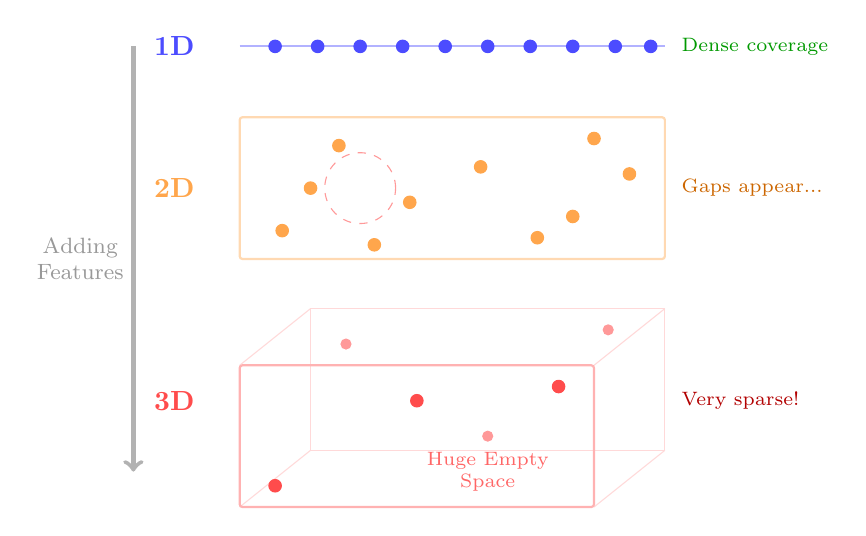
\begin{tikzpicture}[scale=0.9] 
        % --- 1D Line ---
        \node[left, font=\bfseries, blue!70] at (-0.5, 3) {1D};
        \draw[thick, blue!30] (0,3) -- (6,3);
        % 10 points
        \foreach \x in {0.5, 1.1, 1.7, 2.3, 2.9, 3.5, 4.1, 4.7, 5.3, 5.8} 
            \filldraw[blue!70] (\x, 3) circle (2.5pt);
        \node[right, font=\scriptsize, green!60!black] at (6.1, 3) {Dense coverage \checkmark};
        
        % --- 2D Square ---
        \node[left, font=\bfseries, orange!70] at (-0.5, 1) {2D};
        \draw[thick, orange!30, rounded corners=1pt] (0,0) rectangle (6,2);
        % 10 points scattered
        \filldraw[orange!70] (0.6, 0.4) circle (2.5pt);
        \filldraw[orange!70] (1.4, 1.6) circle (2.5pt);
        \filldraw[orange!70] (2.4, 0.8) circle (2.5pt);
        \filldraw[orange!70] (3.4, 1.3) circle (2.5pt);
        \filldraw[orange!70] (4.2, 0.3) circle (2.5pt);
        \filldraw[orange!70] (5.0, 1.7) circle (2.5pt);
        \filldraw[orange!70] (1.0, 1.0) circle (2.5pt);
        \filldraw[orange!70] (4.7, 0.6) circle (2.5pt);
        \filldraw[orange!70] (5.5, 1.2) circle (2.5pt);
        \filldraw[orange!70] (1.9, 0.2) circle (2.5pt);
        
        % Show empty regions
        \draw[red!40, dashed] (1.7, 1.0) circle (0.5cm);
        \node[right, font=\scriptsize, orange!80!black] at (6.1, 1) {Gaps appear...};
        
        % --- 3D Cube (FIXED PERSPECTIVE) ---
        \node[left, font=\bfseries, red!70] at (-0.5, -2) {3D};
        
        % 1. Define Coordinates
        % Front Face: (0, -3.5) to (5, -1.5)
        % Back Face: Shifted by (1, 0.8) -> (1, -2.7) to (6, -0.7)
        
        % 2. Draw Back Face (Behind)
        \draw[red!15, thin] (1,-2.7) rectangle (6,-0.7);
        
        % 3. Draw Connecting Lines (Corners to Corners)
        \draw[red!15, thin] (0,-1.5) -- (1,-0.7); % Top-Left
        \draw[red!15, thin] (5,-1.5) -- (6,-0.7); % Top-Right
        \draw[red!15, thin] (0,-3.5) -- (1,-2.7); % Bottom-Left
        \draw[red!15, thin] (5,-3.5) -- (6,-2.7); % Bottom-Right
        
        % 4. Draw Front Face (In Front)
        \draw[thick, red!30, rounded corners=1pt] (0,-3.5) rectangle (5,-1.5);
        
        % 5. Points (Scattered in "Depth")
        \filldraw[red!70] (0.5, -3.2) circle (2.5pt); % Front-ish
        \filldraw[red!70] (4.5, -1.8) circle (2.5pt); % Front-ish
        \filldraw[red!40] (1.5, -1.2) circle (2pt);   % Back-ish (lighter)
        \filldraw[red!40] (3.5, -2.5) circle (2pt);   % Middle
        \filldraw[red!40] (5.2, -1.0) circle (2pt);   % Far Back-Right
        \filldraw[red!70] (2.5, -2.0) circle (2.5pt); % Middle
        
        % 6. Labels
        \node[red!60, font=\scriptsize, align=center] at (3.5, -3.0) {Huge Empty\\Space};
        \node[right, font=\scriptsize, red!70!black] at (6.1, -2) {Very sparse!};
        
        % Vertical Arrow
        \draw[->, ultra thick, gray!60] (-1.5, 3) -- (-1.5, -3);
        \node[left, align=center, font=\footnotesize, gray!80] at (-1.5, 0) {Adding\\Features};
        
    \end{tikzpicture}
\end{frame}


% --- SLIDE 2: THE SOLUTION ---
\begin{frame}{The Curse of Dimensionality}

    \begin{block}{What Happens in High Dimensions?}
        \begin{itemize}
            \item[\textcolor{blue!70}{$\rightarrow$}] \textbf{1D:} 10 points densely cover the line.
            \item[\textcolor{orange!70}{$\rightarrow$}] \textbf{2D:} Same 10 points spread thin $\rightarrow$ gaps appear.
            \item[\textcolor{red!70}{$\rightarrow$}] \textbf{3D:} Mostly empty space $\rightarrow$ the model starts to find fake patterns in the noise just to bridge the gaps.
        \end{itemize}
    \end{block}

\end{frame}

\begin{frame}{The Solution: Feature Selection}

    \begin{block}{What Happens in High Dimensions?}
        \begin{itemize}
            \item[\textcolor{blue!70}{$\rightarrow$}] \textbf{1D:} 10 points densely cover the line.
            \item[\textcolor{orange!70}{$\rightarrow$}] \textbf{2D:} Same 10 points spread thin $\rightarrow$ gaps appear.
            \item[\textcolor{red!70}{$\rightarrow$}] \textbf{3D:} Mostly empty space $\rightarrow$ the model starts to find fake patterns in the noise just to bridge the gaps.
        \end{itemize}
    \end{block}

    \vspace{2em}
    
    \begin{tcolorbox}[colback=green!5, colframe=green!50, arc=3pt, boxrule=1pt]
        \centering
        \large \textbf{The Fix: Feature Selection}
        \vspace{0.5em}
        \normalsize
        \begin{itemize}
            \item Remove irrelevant features (noise) and keep only meaningful signals.
            \item This should push the data back down to lower dimensions where density is high.
        \end{itemize}
    \end{tcolorbox}

\end{frame}


% --- SLIDE 3: SUMMARY CHEAT SHEET ---
\begin{frame}{Summary: Diagnosing \& Fixing}

    \centering
    \renewcommand{\arraystretch}{1.5}
    \begin{table}[]
        \begin{tabular}{l|l|l}
            \hline
            \textbf{Problem} & \textbf{Diagnosis (Loss)} & \textbf{Mitigation (Fix)} \\ \hline
            \textbf{Underfitting} & \textcolor{blue}{Train High}, \textcolor{red}{Val High} & \begin{tabular}[c]{@{}l@{}} $\uparrow$ Increase Complexity \\ $\uparrow$ Add Features \end{tabular} \\ \hline
            \textbf{Overfitting} & \textcolor{blue}{Train Low}, \textcolor{red}{Val High} & \begin{tabular}[c]{@{}l@{}} $\downarrow$ Reduce Complexity \\ $\downarrow$ Remove Noise/Features \\ $\uparrow$ More Data \\ $\rightarrow$ Regularization (Next Days) \end{tabular} \\ \hline
            \textbf{Good Fit} & \textcolor{blue}{Train Low}, \textcolor{red}{Val Low} & \begin{tabular}[c]{@{}l@{}} $\checkmark$ All good! \end{tabular} \\ \hline
        \end{tabular}
    \end{table}

\end{frame}


% --- PART 4: DATA PREPARATION ---
\section{Data Preparation}

% --- SLIDE 1: TRANSITION ---
\begin{frame}{From Theory to Practice}

    \centering
    \large
    \textit{We know that \textbf{Good Data} cures Overfitting.}
    \vspace{0.5em}
    \textit{But real-world data is rarely "Good." It is messy, broken, and chaotic.}

    \vspace{1.5em}
    
    \begin{columns}[T]
        \begin{column}{0.45\textwidth}
            \centering
            \textbf{Raw Data (Reality)}
            \vspace{0.5em}
            \begin{tcolorbox}[colback=gray!10, boxrule=0pt]
                \centering \small
                \texttt{["NaN", "N/A", -500, "Cat"]}
            \end{tcolorbox}
            \small \textcolor{red}{Models crash on this.}
        \end{column}
        
        \begin{column}{0.1\textwidth}
            \centering \vspace{1cm} \Huge $\rightarrow$
        \end{column}
        
        \begin{column}{0.45\textwidth}
            \centering
            \textbf{Clean Data}
            \vspace{0.5em}
            \begin{tcolorbox}[colback=green!10, boxrule=0pt]
                \centering \small
                \texttt{[0.5, 0.2, 0.0, 1.0]}
            \end{tcolorbox}
            \small \textcolor{green!60!black}{Models learn from this.}
        \end{column}
    \end{columns}

\end{frame}

% --- SLIDE 2: EDA (EXPLORATORY DATA ANALYSIS) ---
\begin{frame}{Step 1: EDA (Know Your Data)}

    \begin{block}{Goal}
        Before training, become a \textbf{Detective}. If you feed garbage in, you get garbage out.
    \end{block}

    \vspace{1em}
    
    \begin{columns}[T]
        % Check 1: Target Dist
        \begin{column}{0.48\textwidth}
            \textbf{1. Check Target Distribution}
            \vspace{0.3em}
            \begin{tcolorbox}[colback=blue!5, boxrule=0pt]
                \centering
                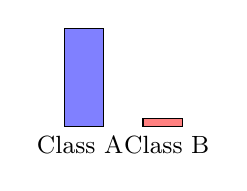
\begin{tikzpicture}[scale=0.5]
                    % Imbalanced
                    \draw[fill=blue!50] (0,0) rectangle (1,2.5); \node[below] at (0.4,0) {\small Class A};
                    \draw[fill=red!50] (2,0) rectangle (3,0.2); \node[below] at (2.6,0) {\small Class B};
                \end{tikzpicture}
                \vspace{0.5em}
                \begin{itemize}
                    \item Is it Imbalanced?
                    \item If yes, use Stratified Split \& F1-Score.
                \end{itemize}
            \end{tcolorbox}
        \end{column}
        
        % Check 2: Red Flags
        \begin{column}{0.48\textwidth}
            \textbf{2. Sanity Checks (Red Flags)}
            \vspace{0.3em}
            \begin{tcolorbox}[colback=red!5, boxrule=0pt]
                \centering
                \small
                \begin{itemize}
                    \item \textbf{Impossible Values:}
                    \item \texttt{Age: -5} $\rightarrow$ \textcolor{red}{Error?}
                    \item \texttt{Age: 200} $\rightarrow$ \textcolor{red}{Outlier?}
                    \item \textbf{Leakage:}
                    \item Does column \texttt{X} perfectly predict \texttt{y}? (e.g., "TransactionID" contains the label).
                \end{itemize}
            \end{tcolorbox}
        \end{column}
    \end{columns}
\end{frame}

% --- SLIDE 3: MISSING VALUES & SCALING ---
\begin{frame}{Step 2: Cleaning \& Scaling}

    \begin{columns}[T]
        % Missing Values
        \begin{column}{0.48\textwidth}
            \textbf{A. Missing Values (NaN)}
            \small Models cannot do math on "Empty".
            \vspace{0.5em}
            \begin{tcolorbox}[colback=gray!5, colframe=gray!50, title=Strategies]
                \small
                \begin{enumerate}
                    \item \textbf{Drop:} Delete the row (only if you have lots of data).
                    \item \textbf{Impute:} Fill with Mean/Median.
                \end{enumerate}
                \vspace{0.5em}
                \centering
                \texttt{[10, ?, 30]} $\rightarrow$ \texttt{[10, \textbf{20}, 30]}
            \end{tcolorbox}
        \end{column}
        
        % Scaling
        \begin{column}{0.55\textwidth}
            \textbf{B. Feature Scaling}
            \small Income (100k) vs. Age (50).
            \vspace{0.5em}
            \begin{tcolorbox}[colback=blue!5, colframe=blue!50, title=Why Scale?]
                \centering
                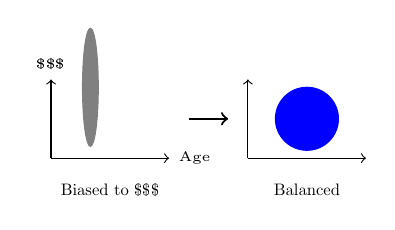
\begin{tikzpicture}[scale=0.5]
                    % Bad Scale
                    \draw[->] (0,0) -- (3,0) node[right] {\tiny Age};
                    \draw[->] (0,0) -- (0,2) node[above] {\tiny \$\$\$};
                    \filldraw[gray] (1, 1.8) ellipse (0.2 and 1.5);
                    \node[scale=0.6] at (1.5, -0.8) {Biased to \$\$\$};
                    
                    % Arrow
                    \draw[->, thick] (3.5, 1) -- (4.5, 1);
                    
                    % Good Scale
                    \draw[->] (5,0) -- (8,0);
                    \draw[->] (5,0) -- (5,2);
                    \filldraw[blue] (6.5, 1) circle (0.8);
                    \node[scale=0.6] at (6.5, -0.8) {Balanced};
                \end{tikzpicture}
                \small
                Models prioritize larger numbers. \\ Scale to $[0,1]$ (Min-Max Scaler) or \\ $\mu=0$, $\sigma=1$ (Standard Scaler).
            \end{tcolorbox}
        \end{column}
    \end{columns}
\end{frame}

% --- SLIDE 4: ENCODING & ENGINEERING ---
\begin{frame}{Step 3: Encoding \& Feature Engineering}

    \begin{columns}[T]
        % Encoding
        \begin{column}{0.48\textwidth}
            \textbf{C. Encoding (Text $\to$ Numbers)}
            \small Models speak Math, not English.
            \vspace{0.5em}
            
            \begin{tcolorbox}[colback=orange!5, boxrule=0pt]
                \textbf{1. Label Encoding} (Ordinal)
                \begin{itemize}
                    \item \texttt{["Low", "High"]} $\to$ \texttt{[0, 1]}
                    \item Use if order matters.
                \end{itemize}
                \vspace{0.3em}
                \textbf{2. One-Hot Encoding} (Nominal)
                \begin{itemize}
                    \item \texttt{["Cat", "Dog"]} $\to$
                    \item \texttt{Cat: [1, 0]}, \texttt{Dog: [0, 1]}
                    \item Use if no order exists.
                \end{itemize}
            \end{tcolorbox}
        \end{column}
        
        % Feature Engineering
        \begin{column}{0.48\textwidth}
            \textbf{D. Feature Engineering}
            \small Creating \textit{new} signals from existing data.
            \vspace{0.5em}
            
            \begin{tcolorbox}[colback=green!5, boxrule=0pt]
                \centering
                \textbf{Example: Date Object}
                \vspace{0.5em}
                
                \texttt{"2023-12-25"}
                \vspace{0.3em}
                \begin{center}
                    $\downarrow$ \textit{Extract Info} $\downarrow$
                \end{center}
                \vspace{0.3em}
                
                \begin{itemize}
                    \item \texttt{Is\_Weekend = 0}
                    \item \texttt{Month = 12} (Winter)
                    \item \texttt{Days\_To\_Holiday = 0}
                \end{itemize}
            \end{tcolorbox}
            \small \textit{This adds value that the raw date string hid.}
        \end{column}
    \end{columns}
\end{frame}

% --- PART 5: MODELING (Teaser) ---
% \section{5. Model Fitting}

% --- SLIDE 1: STEP 4 (TEASER) ---
\begin{frame}{Step 4: Fit the Model}

    \centering
    \large
    \textit{We have clean data. We have robust splits. We have metrics.}
    \vspace{0.3em} % Reduced from 0.5em
    \textbf{Now, we need a model.}
    
    \vspace{0.8em} % Adjusted spacing

    % --- Box 1: The Options ---
    \begin{tcolorbox}[colback=blue!5, colframe=blue!50, title=The Options, width=\textwidth]
        \begin{itemize}
            \item \textbf{Regression:} Linear Regression, Random Forest Regressor...
            \item \textbf{Classification:} Logistic Regression, SVM, Neural Networks...
        \end{itemize}
    \end{tcolorbox}

    \centering
    \begin{block}{}
        \centering
        We will explore \textbf{Machine Learning} \& \textbf{Deep Learning} algorithms in the next sessions!
    \end{block}

\end{frame}

% --- PART 6: SUMMARY ---
\section{References}


\begin{frame}{References}
    \begin{itemize}
        \item Aurélien Géron, \textit{Hands-On Machine Learning with Scikit-Learn, Keras, and TensorFlow}
        \item Andrew Ng, \textit{Machine Learning Specialization} (Coursera/DeepLearning.AI)
    \end{itemize}

    \vspace{2em}
    
    \begin{flushleft}
        \small\textit{Slides contributed by Mohamed Eltayeb}
    \end{flushleft}
    
\end{frame}

